\documentclass[11pt]{article}

\usepackage[T1]{fontenc}
\usepackage{lmodern}
\usepackage{microtype}
\usepackage[a4paper,margin=29mm]{geometry}
\usepackage{amsmath,amssymb,amsthm,mathtools}
\usepackage{booktabs}
\usepackage{enumitem}
\usepackage{array}
\usepackage{float}
\usepackage{xcolor}
\usepackage{tikz}
\usetikzlibrary{arrows.meta,backgrounds,calc,decorations.pathreplacing,
                fit,positioning,shapes.geometric}
\usepackage{hyperref}
\usepackage[nameinlink,capitalise,noabbrev]{cleveref}

\definecolor{ink}{HTML}{17222B}
\definecolor{accent}{HTML}{1F6F78}
\definecolor{accenttwo}{HTML}{C45A3C}
\definecolor{softblue}{HTML}{EAF4F5}
\definecolor{softorange}{HTML}{FBEFE9}
\definecolor{softgray}{HTML}{F3F5F6}
\hypersetup{
  colorlinks=true,
  linkcolor=accent,
  citecolor=accenttwo,
  urlcolor=accent,
  pdftitle={Optimal Local Edge-Set Compression in Regular Graphs},
  pdfsubject={A self-contained exact solution for every regular degree}
}

\setlength{\parindent}{0pt}
\setlength{\parskip}{0.55em}
\setlist{itemsep=0.25em,topsep=0.45em}
\setcounter{tocdepth}{1}
\allowdisplaybreaks

\newtheorem{theorem}{Theorem}[section]
\newtheorem{lemma}[theorem]{Lemma}
\newtheorem{proposition}[theorem]{Proposition}
\newtheorem{corollary}[theorem]{Corollary}
\theoremstyle{definition}
\newtheorem{definition}[theorem]{Definition}
\newtheorem{example}[theorem]{Example}
\theoremstyle{remark}
\newtheorem{remark}[theorem]{Remark}

\newcommand{\bits}{\{0,1\}}
\newcommand{\id}{\operatorname{id}}
\newcommand{\dist}{\operatorname{dist}}
\newcommand{\rank}{\operatorname{rank}}
\newcommand{\outdeg}{\operatorname{outdeg}}
\newcommand{\ceil}[1]{\left\lceil #1\right\rceil}
\newcommand{\floor}[1]{\left\lfloor #1\right\rfloor}
\newcommand{\N}{\mathbb N}

\title{\vspace{-1.2cm}\textbf{Optimal Local Edge-Set Compression\\
in Regular Graphs}}
\author{}
\date{August 2026}

\begin{document}
\maketitle
\vspace{-0.9cm}

\begin{abstract}
Fix a degree $d$.  An omniscient encoder is given a finite simple
$d$-regular graph, unique vertex identifiers, and one arbitrary bit on every
edge.  It writes the same number of bits at every vertex.  A fixed decoder
must recover the bit of a queried edge from a constant-radius neighborhood,
where the radius may depend on $d$ but not on the graph size.  The decoder
is not given the graph size, and identifiers are arbitrary distinct natural
numbers.  We determine
the exact label length for every positive degree:
\[
 b_{\rm reg}(d)=\ceil{(d+1)/2}=\floor{d/2}+1.
\]
For odd $d$ this is the integral counting bound.  For even $d$, counting
suggests $d/2$ bits, but uniform local decoding forces one additional bit.

The construction is explicit and self-contained.  Star-shaped marker words
expose bounded connected Voronoi blocks.  A canonical in-block matching gives a
self-synchronizing high-rate block code.  After canceling parallel boundary
edges in opposite pairs, paired incidences turn the remaining quotient into
virtual paths and cycles.  A small part of the block-code surplus stores
occasional absolute direction records on these paths and cycles.  A finite
capacitated Hall argument places the records densely enough for local
decoding, while the induced orientation makes every block own at most half
of its boundary edges, up to rounding.  No local orientation theorem, Lov\'asz
Local Lemma, or prior compression scheme is used as a black box.  The even
lower bound uses zero-slack circulant strips.  Finite-ring surjectivity makes
their induced maps reversible; reflection moves an odd total number of binary
edge tracks, contradicting a self-contained rational information-flow index.
With simple uniform constants the upper-bound radius is $O(d^5\log d)$ for
$d\ge3$; for cubic graphs it is $1{,}007{,}136{,}282$.
\end{abstract}

\tableofcontents

\section{Introduction}

Local computation usually asks what a network can compute after a bounded
number of communication rounds.  Here the network additionally receives a
short, instance-dependent label at each vertex.  The labels may be chosen by
an unrestricted centralized encoder, but the decompressor must be one fixed
local rule.  This ``local advice and decompression'' viewpoint was formulated
for graph problems by Balliu et al.~\cite{BalliuEtAl2024Brief,
BalliuEtAl2025LocalAdvice}; it sits within the broader traditions of the
LOCAL model~\cite{NaorStockmeyer1995} and distributed computation with
advice~\cite{FraigniaudEtAl2009Advice}.

We study the cleanest lossless compression problem in this model.  Each edge
of a known graph carries an arbitrary hidden bit---equivalently, the hidden
object is an arbitrary subset of the edges.  The topology and unique vertex
identifiers are free side information.  Labels are placed on vertices, and
the bit of each edge must be readable nearby.

On an $n$-vertex $d$-regular graph there are $dn/2$ independent edge bits.
Thus labels of $s$ bits per vertex can work only if $sn\ge dn/2$.  For odd
$d$, integrality gives $s\ge(d+1)/2$.  For even $d$, this elementary argument
only gives $s\ge d/2$.  Balliu et al.~\cite{BalliuEtAl2025LocalAdvice} gave a
general upper bound one bit above the integral counting lower bound and singled
out the cubic two-bit case.  Our construction answers that cubic question.
For the graph-size-independent decoding model defined below, we also determine
the optimum in every regular degree: constructive entropy sharing settles
the odd degrees, and a reversible one-dimensional index rules out the
zero-slack rate in the positive even degrees.

Several neighboring source-coding models use similar terminology but differ
from this worst-case graph-metric game.  Makhdoumi et al. study recovery of
source coordinates by probing selected coordinates of a globally compressed
random sequence~\cite{MakhdoumiEtAl2015LDSC}, while Vatedka, Chandar, and
Tchamkerten study separately encoded correlated random
sources~\cite{VatedkaEtAl2022LocalDecoding}.  Delgosha and Anantharam study
asymptotic compression of random marked sparse graphs and universal
compression of the graph and its marks~\cite{DelgoshaAnantharam2022DistributedGraphical,
DelgoshaAnantharam2020UniversalGraphical}.  Here the graph is uncompressed
side information, the edge bits are arbitrary, storage is uniformly bounded
at every vertex, access is restricted to a bounded graph-distance view, and
recovery is exact on every finite instance.  Thus these works are adjacent
context, not prior bounds for this model.  Certificate--radius
tradeoffs~\cite{FeuilloleyEtAl2021Redundancy}, distributed degree
splitting~\cite{GhaffariEtAl2020DegreeSplitting}, sinkless-orientation
locality~\cite{BalliuEtAl2023Sinkless}, and distributed versions of Hall's
theorem~\cite{BrandtEtAl2025Hall} provide further methodological context;
none is a proof dependency, and our matching use is ordinary finite Hall at
the centralized encoder.

\begin{quote}
\textbf{Main result, informally.}
For every $d\ge1$, exactly $\ceil{(d+1)/2}$ bits per vertex are necessary and
sufficient to locally encode every edge subset of every finite simple
$d$-regular graph.  Odd degrees attain counting; even degrees require one
bit more than counting.
\end{quote}

The apparent obstacle is ownership.  If every edge has one endpoint that
``owns'' it, that endpoint can store its bit.  At the counting optimum, a
block of $b$ vertices has room for only about $db/2$ owned edges.  Hence its
boundary edges must be directed almost evenly in and out.  A globally chosen
balanced orientation is easy to imagine but is not free side information;
the decoder must reconstruct it from the same optimal-length labels that
carry the payload.

Our construction uses the at-least-half-bit-per-vertex margin between
$d/2$ and $\ceil{(d+1)/2}$.  Large components are partitioned into bounded connected
blocks, each marked by a recognizable star.  The nonmarker labels form a
product code with linear entropy surplus after reserving $\ceil{db/2}$
payload bits.  We use that surplus for sparse 
\emph{direction records}.  At the quotient level, a purely combinatorial
incidence pairing decomposes the orientation problem into paths and cycles.
One nearby record fixes the direction of an entire visible segment.  A
capacitated Hall argument guarantees that records can be stored by the
blocks occurring in those segments.  The Hall theorem needed for this step
is proved in full in \cref{lem:capacitated-hall}.

The resulting proof is insensitive to expansion, girth, bridges, and block
shape.  A block may look like a tree, a ladder, or an arbitrary connected
subgraph.  Components too small to amortize a marker use a direct code, and a
component contained in one large block simply has no quotient boundary.

\paragraph{Organization.}
\Cref{sec:model} fixes the exact decoding model and states the theorem.
\Cref{sec:overview} gives a visual proof overview.  Self-exposing blocks and
their finite code are built in \cref{sec:blocks}.  The quotient orientation
skeleton appears in \cref{sec:quotient}; record capacity and placement are
proved in \cref{sec:capacity,sec:records}.  The encoder and a total decoder
on \emph{all} labeled inputs are specified in
\cref{sec:encoder,sec:decoder}.  \Cref{sec:locality} proves the radius bound.
Order normalization,
finite-ring reversibility, the rational flow index, and the even-degree
obstruction are proved in
\cref{sec:normalization,sec:index,sec:even-lower}.  Finally,
\cref{sec:conclusion} assembles the exact all-degree theorem.

\section{Model and statement of the theorem}
\label{sec:model}

Input graphs are finite, undirected, and simple; they may be disconnected
or empty.  Infinite graphs occur only as auxiliary objects in the lower
bound.  Fix a degree $d$.  An input consists of a $d$-regular graph
$G=(V,E)$, an injective identifier map $\id:V\to\N$, and a target vector
$x\in\bits^E$.  Identifiers and the topology are visible to both encoder and
decoder and are not charged to the label length.  Whenever an order of
incident edges is needed, we use increasing neighbor identifier, so no
additional port numbering is required.
Graph distances take the value $+\infty$ between different components.

For an edge $e=uv$, its radius-$r$ edge ball has vertex set
\[
 V_r(G,e)=\{w\in V:\min\{\dist(w,u),\dist(w,v)\}\le r\}.
\]
For a labeling $\ell:V\to\Sigma$, write
$\mathsf{View}_r(G,\id,\ell,e)$ for the finite rooted structure consisting of
the edge $e$, the subgraph induced by $V_r(G,e)$, the restrictions of $\id$
and $\ell$ to this vertex set, and the following exact port table.  The
visible vertices are indexed canonically in increasing identifier order.  At
each visible vertex, the $d$ ports are indexed by the identifier order of all
its global neighbors.  A port contains the corresponding local vertex when
that neighbor is visible and an opaque stub otherwise.  A stub reveals its
port position, but no outside endpoint, identifier, label, or adjacency.

The decoder is a total function on the corresponding raw finite structures,
not merely on structures that arise by extraction.  Thus its input may have
repeated identifiers or an inconsistent port table; the local graph is still
simple, the root is still an actual local edge, and every label is still an
element of $\Sigma$.  Correctness is required only on the genuine extracted
views just defined.  This is the precise edge-view convention used throughout.
Raw structures need not satisfy the extracted view's degree, size,
connectedness, or root-distance constraints.

\begin{definition}[Local edge-set code]
Let $\Sigma$ be a finite alphabet.  A radius-$r$ decoder is one fixed,
deterministic, total function $D$ that maps every $\Sigma$-labeled rooted
radius-$r$ edge view to a bit.  It is valid for $d$-regular graphs if
\[
 \forall G\;\forall\id\;\forall x\in\bits^{E(G)}\;
 \exists\ell:V(G)\to\Sigma\;\forall e\in E(G):
 D\bigl(\mathsf{View}_r(G,\id,\ell,e)\bigr)=x_e.              \tag{2.1}
\]
The encoder choosing $\ell$ is centralized and computationally unrestricted.
It need not be local, canonical, or efficient.  The decoder is not told the
component size or the global number of vertices.
\end{definition}

In particular, the quantifier order is $\exists r\,\exists D$ followed by
the universal quantifiers in (2.1).  The same $D$ must work at every graph
size and for every injective natural-number identifier assignment.  This
differs from versions of the LOCAL model in which vertices are supplied
with the global size $n$ or identifiers are restricted to a prescribed
polynomial-size range.  Our bit upper bound applies to those models as
well: an endpoint can gather the edge view and the neighbor layer defining
its ports in at most $r+2$ communication rounds for a radius-$r$ rule, then simulate the same
edge-rooted decoder.  The two endpoints obtain identical outputs.
The counting lower bound still applies.  The even-degree
lower bound proved here is for (2.1); we do not claim its extension to a
decoder supplied with $n$ or to a restricted identifier range.

For $s\in\N$, labels of $s$ bits mean an alphabet of exactly $2^s$ symbols.
Let $b_{\mathrm{reg}}(d)$ be the least $s$ for which some finite radius and
some decoder satisfy (2.1) for every finite simple $d$-regular graph.
Equivalently, for each fixed graph and identifier assignment, the global map
induced by applying $D$ at every edge must be onto $\bits^E$.
This minimum exists: $d$ bits always suffice by storing each incident edge
bit in its port position and reading it at the lower-identifier endpoint.
On raw views it breaks identifier ties by local vertex index, uses the
first port pointing to the other root endpoint, and returns zero if no
such port exists.

All logarithms below are base two.  For every $d\ge3$, define
\begin{equation}
 \begin{aligned}
 s_d&=\ceil{\frac{d+1}{2}}, & \alpha_d&=2^{s_d},\\[-1mm]
 \Sigma_d&=\{0,1,\ldots,\alpha_d-1\}.&&
 \end{aligned}                                                \tag{2.2}
\end{equation}
\begin{align}
 b_\star&=64(d+1)^2, & \eta&=2b_\star-2,                     \tag{2.3}\\
 B_{\max}&=1+d\sum_{j=0}^{\eta-1}(d-1)^j
   =1+\frac d{d-2}\bigl((d-1)^\eta-1\bigr),                 \tag{2.4}\\
 \chi_d&=\ceil{\log_2(dB_{\max})},
 &L&=20d\chi_d,                                               \tag{2.5}\\
 R_d&=(2L+3)(2\eta+2).                                       \tag{2.6}
\end{align}
The letter $L$ is the length of a virtual record window, not the length of a
physical label.  The constants depend only on $d$; their roles are summarized
below.

\begin{center}
\small
\renewcommand{\arraystretch}{1.08}
\begin{tabular}{@{}>{$}c<{$}@{\qquad}l@{}}
\toprule
\text{parameter} & \text{purpose}\\
\midrule
b_\star & minimum size at which a marker is amortized\\
\eta & domination radius and malformed-input cutoff\\
B_{\max} & uniform upper bound on a parsed block size\\
\chi_d & uniform upper bound on a record width\\
L & length of a virtual window\\
R_d & advertised physical decoding radius\\
\bottomrule
\end{tabular}
\end{center}

\begin{theorem}[Optimal compression in every regular degree]
\label{thm:main}
For every $d\ge3$, there is a deterministic radius-$R_d$ decoder over
$\Sigma_d$ satisfying (2.1).  Consequently,
\[
 b_{\mathrm{reg}}(d)=\ceil{\frac{d+1}{2}}
                    =\floor{\frac d2}+1
 \qquad(d\ge1).                                             \tag{2.7}
\]
For $d=3$, the displayed construction has
\[
                         R_3=1{,}007{,}136{,}282.              \tag{2.8}
\]
The edgeless case has $b_{\mathrm{reg}}(0)=0$.
\end{theorem}

The upper bounds for $d=1,2$ use the direct codes described in
\cref{sec:conclusion}; the even-degree lower-bound argument also includes
$d=2$.  In the upper-bound construction below, $d\ge3$ and all constants
are those in (2.2)--(2.6).  Ceilings of logarithms may always be evaluated by
integer comparisons; no real arithmetic is required of the decoder.

\section{Proof idea}
\label{sec:overview}

The information budget is easiest to see blockwise.  Let $E(B)$ be the set
of edges with both endpoints in a block $B$, let $\partial B$ be its edge
boundary, and put $b=|B|$.  Regularity gives
$db=2|E(B)|+|\partial B|$.  The average target-bit budget at the counting
rate is $db/2$.  If $B$ owns every internal edge and at most half of its
boundary edges (rounded up), then it owns at most
\[
   |E(B)|+\ceil{\frac{|\partial B|}{2}}=\ceil{\frac{db}{2}}
\]
edges.  These are the payload bits that $B$ must store.

\Cref{fig:pipeline} summarizes the construction.  Every step is locally
reconstructible on a valid encoding.  In particular, the decoder discovers
the blocks from the physical labels before it interprets their logical
contents, so there is no circular use of hidden metadata.

\begin{figure}[H]
\centering
\resizebox{0.96\linewidth}{!}{%
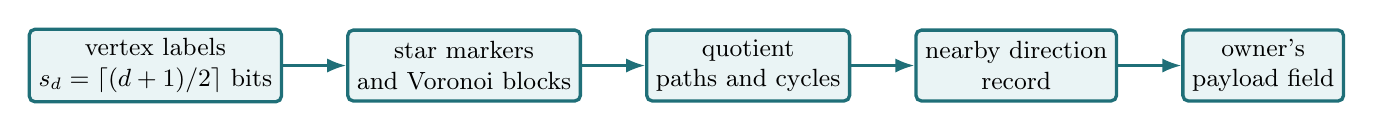
\begin{tikzpicture}[
  box/.style={draw=accent,very thick,rounded corners=2pt,fill=softblue,
              minimum height=9mm,align=center,font=\small},
  arr/.style={-{Latex[length=2.4mm]},thick,accent}
]
\node[box] (labels) {vertex labels\\$s_d=\lceil(d+1)/2\rceil$ bits};
\node[box,right=8mm of labels] (blocks) {star markers\\and Voronoi blocks};
\node[box,right=8mm of blocks] (strands) {quotient\\paths and cycles};
\node[box,right=8mm of strands] (records) {nearby direction\\record};
\node[box,right=8mm of records] (payload) {owner's\\payload field};
\draw[arr] (labels)--(blocks);
\draw[arr] (blocks)--(strands);
\draw[arr] (strands)--(records);
\draw[arr] (records)--(payload);
\end{tikzpicture}%
}
\caption{The decoder's dependency chain.  Window boundaries and the Hall
assignment are encoder-side devices; the decoder only needs their explicit
nearby records.}
\label{fig:pipeline}
\end{figure}

Why is there room for structural information?  The marker uses a bounded
number of vertices in a large block.  On the other vertices, even the
restricted alphabet $\Sigma_d\setminus\{1\}$ carries
$\log_2(2^{s_d}-1)>d/2$ bits per vertex.  After marker losses and integer
rounding, we retain at least $b/20$ extra logical bits in every block.  These
bits are split into record slots.

To balance boundary ownership, parallel quotient edges are first canceled
in oppositely directed pairs.  The remaining quotient is simple.  At every
quotient vertex, pair consecutive incidences.  Splitting a vertex according
to these pairs turns the quotient into disjoint paths and cycles.  Directing
each path or cycle consistently makes every paired copy have one incoming
and one outgoing edge; only a possible singleton can be unbalanced.  Sparse
absolute records make this direction locally recoverable.  The capacity
argument is global only at encoding time: Hall's theorem assigns each
length-$L$ path window to a record slot of a block occurring in it.

\section{Self-exposing blocks and their code}
\label{sec:blocks}

We begin with a connected component containing at least $b_\star$ vertices.
Small components will be encoded directly in \cref{sec:encoder}.

\subsection{Bounded connected Voronoi blocks}

The encoder chooses an inclusion-maximal set $\mathcal C$ of vertices whose
distinct members have pairwise distance at least
\[
                            2b_\star-1=\eta+1.                 \tag{4.1}
\]
Such a set exists because the component is finite.  Maximality implies that
every vertex is within distance $\eta$ of $\mathcal C$: otherwise that vertex
could be added.  Assign each vertex $v$ to the center $c\in\mathcal C$ that
minimizes
\[
                            (\dist(v,c),\id(c))                 \tag{4.2}
\]
lexicographically.  Write $B_c$ for the resulting block.

\begin{lemma}[Block geometry]
\label{lem:block-geometry}
Every $B_c$ is connected, contains the closed neighborhood $N[c]$, and has
\[
                            b_\star\le |B_c|\le B_{\max}.       \tag{4.3}
\]
\end{lemma}

\begin{proof}
Domination puts $B_c$ inside the radius-$\eta$ ball about $c$.  A graph of
maximum degree $d$ has at most
$1+d\sum_{j=0}^{\eta-1}(d-1)^j=B_{\max}$ vertices in such a ball, proving the
upper bound: a shortest path has at most $d$ choices for its first edge
and at most $d-1$ choices at each later step, since it cannot immediately
return along the preceding edge.

If $\dist(v,c)\le b_\star-1$ and $c'\ne c$ is another center, then
\[
 \dist(v,c')\ge \dist(c,c')-\dist(v,c)
              \ge(2b_\star-1)-(b_\star-1)=b_\star.
\]
Thus $v$ is strictly closer to $c$ than to every other center.  The entire
radius-$(b_\star-1)$ ball about $c$ lies in $B_c$.  This ball has at least
$b_\star$ vertices: if a geodesic of length $b_\star-1$ exists, take its
vertices; otherwise the ball is the whole component, which by assumption
has at least $b_\star$ vertices.  This also gives $N[c]\subseteq B_c$.

For connectedness, let $v\in B_c$, and let $w$ be the next vertex on a
shortest $v$--$c$ path.  If a center $c'$ beat $c$ in the lexicographic rule
at $w$, then $\dist(v,c')\le\dist(w,c')+1$.  A strict distance advantage at
$w$ remains an advantage at $v$; in the tied-distance case, the same
identifier tie-break also makes $c'$ beat $c$ at $v$.  Both contradict
$v\in B_c$.  Hence $w\in B_c$, and iteration gives a path from $v$ to $c$
inside $B_c$.
\end{proof}

The argument includes the case in which the entire component is one block.
No growth or expansion assumption was used.

\subsection{A marker that cannot be forged by data}

Set $\alpha=\alpha_d$ and $\Sigma=\Sigma_d$ for brevity.  A vertex is called
a \emph{marked center} when its label is $1$ and all its $d$ neighbors have
label $0$.  In an intended block $B=B_c$, the encoder fixes label $1$ at $c$
and label $0$ at every vertex in $N(c)$.  The data region is
\[
                    F_B=B\setminus N[c],\qquad
                    r_B=|F_B|=|B|-d-1.                         \tag{4.4}
\]

Order all graph edges by the globally unique key
\[
 \kappa(uv)=\bigl(\min\{\id(u),\id(v)\},
                   \max\{\id(u),\id(v)\}\bigr).              \tag{4.5}
\]
Run the greedy matching algorithm on the induced graph $G[F_B]$, processing
edges in increasing $\kappa$ order.  This gives a canonical maximal
\emph{buddy matching} $M_B$; put $m_B=|M_B|$.  Order the endpoints of every
matched edge by identifier.  A word on $F_B$ is \emph{legal} when
\begin{itemize}
\item an unmatched vertex receives any symbol except $1$; and
\item a matched ordered pair receives any element of $\Sigma^2$ except
      $(1,0)$ and $(0,1)$.
\end{itemize}
Therefore the exact number of legal data words is
\[
                N_B=(\alpha^2-2)^{m_B}
                     (\alpha-1)^{r_B-2m_B}.                    \tag{4.6}
\]

\begin{figure}[H]
\centering
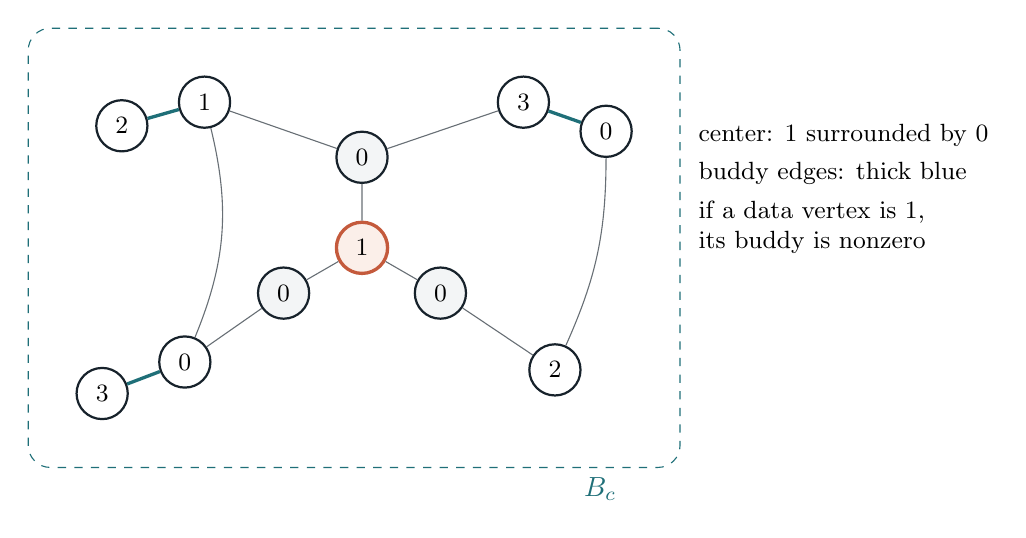
\begin{tikzpicture}[
  v/.style={circle,draw=ink,thick,minimum size=6.5mm,inner sep=0pt,
            font=\small},
  zero/.style={v,fill=softgray},
  center/.style={v,fill=softorange,draw=accenttwo,very thick},
  data/.style={v,fill=white},
  buddy/.style={very thick,accent},
  edge/.style={thin,ink!65}
]
\node[center] (c) at (0,0) {$1$};
\node[zero] (z1) at (90:1.15) {$0$};
\node[zero] (z2) at (210:1.15) {$0$};
\node[zero] (z3) at (330:1.15) {$0$};
\draw[edge] (c)--(z1) (c)--(z2) (c)--(z3);

\node[data] (a) at (-2.0,1.85) {$1$};
\node[data] (b) at (-3.05,1.55) {$2$};
\node[data] (d) at (2.05,1.85) {$3$};
\node[data] (e) at (3.10,1.48) {$0$};
\node[data] (f) at (-2.25,-1.45) {$0$};
\node[data] (g) at (-3.30,-1.85) {$3$};
\node[data] (u) at (2.45,-1.55) {$2$};
\draw[edge] (z1)--(a) (z1)--(d) (z2)--(f) (z3)--(u);
\draw[buddy] (a)--(b) (d)--(e) (f)--(g);
\draw[edge] (a) to[bend left=18] (f) (e) to[bend left=12] (u);
\begin{scope}[on background layer]
\node[draw=accent,dashed,rounded corners=8pt,fit=(c)(z1)(z2)(z3)(a)(b)(d)(e)(f)(g)(u),
      inner sep=6mm,label={[accent]below right:$B_c$}] {};
\end{scope}
\node[align=left,font=\small,anchor=west] at (4.15,0.75)
  {center: $1$ surrounded by $0$\\[1mm]
   buddy edges: thick blue\\[1mm]
   if a data vertex is $1$,\\its buddy is nonzero};
\end{tikzpicture}
\caption{A schematic cubic block, where $\Sigma=\{0,1,2,3\}$.  Only edges
relevant to the marker and sample buddy pairs are shown; omitted incidences
continue inside or outside the block.  The drawing is not to scale: an actual
large block has at least $1024$ vertices.  The displayed data labels are one
legal word.  On each buddy edge all $16$ ordered pairs except $(1,0)$ and
$(0,1)$ are permitted.}
\label{fig:star-buddy}
\end{figure}

\begin{lemma}[Self-synchronization and code size]
\label{lem:star-code}
In a legal block word, the center $c$ is the only marked center in $B$.
Moreover,
\[
                             N_B\ge(\alpha-1)^{|B|-d-1}.        \tag{4.7}
\]
\end{lemma}

\begin{proof}
The vertex $c$ is marked by construction, and its neighbors have label zero.
An unmatched data vertex cannot have label $1$.  If a matched data vertex has
label $1$, its buddy is an actual graph neighbor and is nonzero, by the two
forbidden pairs.  It therefore cannot be marked.  These cases cover $B$.

For the count, observe that
\[
 \alpha^2-2-(\alpha-1)^2=2\alpha-3>0
\]
because $\alpha\ge4$.  Replacing every matched-pair factor in (4.6) by
$(\alpha-1)^2$ proves (4.7).
\end{proof}

Fix once and for all increasing orders of the $\alpha-1$ unmatched symbols
and lexicographic order of the $\alpha^2-2$ legal ordered pairs.  Together with increasing
identifier order of unmatched vertices and increasing $\kappa$ order of
matching edges, the block topology and identifiers determine a mixed-radix
enumeration
\[
              \{0,1,\ldots,N_B-1\}
                 \longleftrightarrow
              \{\text{legal words on }F_B\}.                  \tag{4.8}
\]
For definiteness, list the matched-edge coordinates first and the unmatched
vertices second.  If their radices are $r_0,\ldots,r_{u-1}$ and their
zero-based symbol ranks are $a_0,\ldots,a_{u-1}$, the word rank is
$\sum_{i=0}^{u-1}a_i\prod_{j<i}r_j$.  Successive Euclidean divisions give
the inverse map.  Empty products equal one and empty sums equal zero.
Unranking an integer through this enumeration is a finite, explicit operation
on the topology and identifiers.  Ranking is its inverse and additionally
reads the physical symbols on $F_B$.

Applying \cref{lem:star-code} to all blocks shows that the marked centers in
the completed physical labeling are \emph{exactly} $\mathcal C$.  Hence a
decoder first detects the stars, then repeats (4.2), and reconstructs the
same blocks and buddy matchings.  The logical contents of (4.8) are not used
to discover the blocks.

\subsection{Linear structural surplus}

For a block of size $b=|B|$, reserve
\[
                    \pi_B=\ceil{\frac{db}{2}}                 \tag{4.9}
\]
payload coordinates.  We use the following conservative whole-bit budget
and its remaining structural surplus:
\[
                    c_B=\floor{\log_2((\alpha-1)^{b-d-1})},\qquad
                    \sigma_B=c_B-\pi_B.                       \tag{4.10}
\]
By (4.7), $2^{c_B}\le N_B$.  The exact legal-word count $N_B$ is used for
physical ranking and unranking, but all field lengths use the budget
$c_B$ in (4.10), not $\floor{\log_2N_B}$.  Thus the field lengths depend
only on $d$, $b$, and the residual degree defined below.

\begin{lemma}[Uniform surplus]
\label{lem:surplus}
Every block produced above satisfies
\[
                              \sigma_B\ge\frac{|B|}{20}.        \tag{4.11}
\]
\end{lemma}

\begin{proof}
Write $s=s_d=\ceil{(d+1)/2}$.  On integers $s\ge2$, the function
\[
 f(s)=\log_2(2^s-1)-(s-1/2)
\]
is increasing, because
\[
 f(s+1)-f(s)=
 \log_2\!\left(\frac{2^{s+1}-1}{2(2^s-1)}\right)>0.
\]
Also $3^{16}=43{,}046{,}721>33{,}554{,}432=2^{25}$, so
$f(2)>1/16$.  Since $s\ge(d+1)/2$, this yields, for every $d\ge3$,
\[
                    \log_2(\alpha-1)\ge\frac d2+\frac1{16}.   \tag{4.12}
\]
By (4.10), $\floor y\ge y-1$, and
$\ceil{db/2}\le db/2+1/2$,
\begin{align*}
 \sigma_B
 &\ge (b-d-1)\left(\frac d2+\frac1{16}\right)
       -1-\frac{db}{2}-\frac12\\
 &=\frac b{16}-(d+1)\left(\frac d2+\frac1{16}\right)-\frac32\\
 &\ge\frac b{16}-\frac{(d+1)^2}{2}-\frac32.
\end{align*}
Because $b\ge b_\star=64(d+1)^2$, the middle loss is at most $b/128$.
Furthermore $b\ge1024>320$, so $3/2\le3b/640$.  Consequently
\[
 \sigma_B\ge\frac b{16}-\frac b{128}-\frac{3b}{640}
             =\frac b{20}.
\]
\end{proof}

The budget deliberately leaves the positive rate improvement from buddy
pairs unused.  It therefore covers every connected block shape, even one
whose data region has a very small matching.  The matching permits symbol
$1$ at matched data vertices without creating false markers; the resulting
larger physical code is still enumerated exactly by (4.8).

\section{From the block quotient to virtual strands}
\label{sec:quotient}

Fix the encoder-produced blocks in one large connected component.  The quotient
multigraph $J$ has one vertex for every block.  Every original edge whose
endpoints lie in different blocks gives one edge of $J$; internal edges do
not enter $J$ and hence create no loops.

For the rest of the construction, write $z_B$ for the marked center of a
physical block $B$.

For each unordered pair of blocks, sort its parallel quotient edges by the
original-edge key $\kappa$ from (4.5), pair consecutive edges, and delete
each pair from the residual quotient.  In a deleted pair, direct the first
edge from the lower-identifier center to the higher-identifier center and
the second in the reverse direction.  If the multiplicity is odd, its last
edge remains.  Thus the residual quotient $K$ is finite, simple, and
loopless.  Isolated quotient vertices are allowed.

Let $k_B$ be the degree of $B$ in $K$.  Since $K$ is simple, the identifiers
of the centers at the other endpoints give a tie-free order of the
incidences at $B$.  Pair incidences $(1,2),(3,4),\ldots$, leaving the last
one single if $k_B$ is odd.  Split $B$ into one \emph{virtual copy} for every
pair or singleton.  Each edge of $K$ now joins the copies containing its two
incidences.  Call the resulting graph $H$.  The number of copies above $B$
is
\[
                         \nu_B=\ceil{\frac{k_B}{2}}.            \tag{5.1}
\]
Index them in incidence order, and give the $j$th copy the key
$(\id(z_B),j)$.  Paired copies have degree two and singleton copies have
degree one; if $k_B=0$, there is no copy.  Hence $H$ is a disjoint union of
finite paths and cycles.  Indeed, a walk starting at a degree-one vertex
has a unique continuation at each internal vertex and ends at the other
degree-one vertex; connectedness leaves no additional vertices in that
component.  A component without a degree-one vertex is finite and
two-regular, so following successive edges returns to the starting vertex
and exhausts a cycle.  The same physical block may occur through several
virtual copies, possibly on the same component of $H$.  We call the
components of $H$ \emph{virtual strands}.

\begin{figure}[H]
\centering
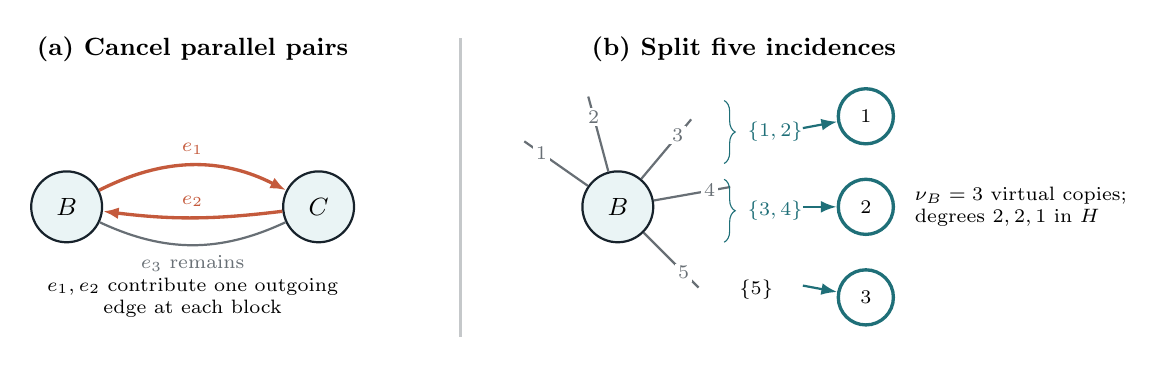
\begin{tikzpicture}[
  qv/.style={circle,draw=ink,thick,fill=softblue,minimum size=9mm,
             inner sep=0pt,font=\small},
  vv/.style={circle,draw=accent,very thick,fill=white,minimum size=7mm,
             inner sep=0pt,font=\scriptsize},
  ed/.style={thick,ink!65},
  can/.style={-{Latex[length=2mm]},very thick,accenttwo}
]
\node[font=\small\bfseries] at (-3.4,2.0) {(a) Cancel parallel pairs};
\node[qv] (B) at (-5.0,0) {$B$};
\node[qv] (C) at (-1.8,0) {$C$};
\draw[can] (B) to[bend left=27] node[above,font=\scriptsize] {$e_1$} (C);
\draw[can] (C) to[bend left=7] node[above,font=\scriptsize] {$e_2$} (B);
\draw[ed] (B) to[bend right=25] node[below,font=\scriptsize] {$e_3$ remains} (C);
\node[font=\scriptsize,align=center] at (-3.4,-1.15)
  {$e_1,e_2$ contribute one outgoing\\edge at each block};

\draw[ink!25,very thick] (0,-1.65)--(0,2.15);
\node[font=\small\bfseries] at (3.6,2.0) {(b) Split five incidences};
\node[qv] (D) at (2.0,0) {$B$};
\foreach \i/\ang in {1/145,2/105,3/50,4/10,5/-45}{
  \coordinate (p\i) at ($(D)+(\ang:1.45)$);
  \draw[ed] (D)--(p\i) node[pos=.73,fill=white,inner sep=1pt,font=\scriptsize] {$\i$};
}
\node[vv] (x1) at (5.15,1.15) {$1$};
\node[vv] (x2) at (5.15,0) {$2$};
\node[vv] (x3) at (5.15,-1.15) {$3$};
\draw[decorate,decoration={brace,amplitude=4pt},accent]
  (3.35,1.35)--(3.35,.55) node[midway,right=5pt,font=\scriptsize] {$\{1,2\}$};
\draw[decorate,decoration={brace,amplitude=4pt},accent]
  (3.35,.35)--(3.35,-.45) node[midway,right=5pt,font=\scriptsize] {$\{3,4\}$};
\node[font=\scriptsize,anchor=west] at (3.42,-1.05) {$\{5\}$};
\draw[-{Latex[length=2mm]},accent,thick] (4.35,1.0)--(x1);
\draw[-{Latex[length=2mm]},accent,thick] (4.35,0)--(x2);
\draw[-{Latex[length=2mm]},accent,thick] (4.35,-1.0)--(x3);
\node[font=\scriptsize,align=left,anchor=west] at (5.65,0)
  {$\nu_B=3$ virtual copies;\\degrees $2,2,1$ in $H$};
\end{tikzpicture}
\caption{The quotient reduction.  Oppositely directed parallel pairs are
already balanced.  Pairing the remaining incidences turns the residual
orientation problem into paths and cycles.}
\label{fig:quotient}
\end{figure}

A \emph{consistent direction} of an $H$-path directs all edges from one
endpoint to the other; on an $H$-cycle it chooses one of the two cyclic
directions.  Transferring these directions back to $K$ gives the following
elementary bound.

\begin{lemma}[Balanced quotient ownership]
\label{lem:ownership}
If every component of $H$ is directed consistently, then
\[
                       \outdeg_K(B)\le\nu_B
                         =\ceil{\frac{k_B}{2}}.                 \tag{5.2}
\]
After the canceled pairs are restored, direct each original interblock edge
as above or as prescribed by $K$.  If $B$ owns its internal edges and its
outgoing interblock edges, then it owns at most $\pi_B=\ceil{d|B|/2}$ edges.
Every original edge has exactly one owner.
\end{lemma}

\begin{proof}
At a paired virtual copy, a consistent path or cycle direction has one
incoming and one outgoing incidence.  Only a singleton copy can contribute
an unmatched outgoing incidence.  Thus every copy contributes at most one
outgoing edge at its physical block, proving (5.2).

Let $i_B$ and $\delta_B$ be the numbers of internal and boundary edges of
$B$.  Removing parallel pairs deletes an even number of incidences at $B$,
so $\delta_B\equiv k_B\pmod2$.  The removed pairs contribute exactly
$(\delta_B-k_B)/2$ outgoing edges at $B$.  Therefore the total number of
outgoing boundary edges is at most
\[
 \frac{\delta_B-k_B}{2}+\ceil{\frac{k_B}{2}}
   =\ceil{\frac{\delta_B}{2}}.                                \tag{5.3}
\]
Regularity gives $2i_B+\delta_B=d|B|$, and hence
\[
 i_B+\ceil{\frac{\delta_B}{2}}
   =\ceil{\frac{d|B|}{2}}=\pi_B.                              \tag{5.4}
\]
Internal edges have their unique block as owner, and every interblock edge
has exactly one tail, so ownership partitions $E(G)$.
\end{proof}

Bridges merely appear on virtual paths and need no special treatment.  If a
whole component is one block, then $K$ and $H$ are empty and the lemma says
that all internal edges fit in the ordinary payload.

\section{How many direction records fit?}
\label{sec:capacity}

The orientation of $H$ has not yet been made locally visible.  A record
stored by $B$ will be either empty or will name one of its $\nu_B$ virtual
copies and specify whether a fixed reference incidence at that copy points
out of or into $B$.  For a paired copy, take its first incidence in the local
order as reference; for a singleton, take its unique incidence.  Thus there
are $2\nu_B+1$ record states.

When $k_B>0$, define the record width and number of available slots by
\[
 w_B=\ceil{\log_2(2\nu_B+1)},\qquad
 t_B=\floor{\frac{\sigma_B}{w_B}}.                             \tag{6.1}
\]
When $k_B=0$, set $\nu_B=w_B=t_B=0$.  In $w_B$ bits, value $0$ means empty;
for $1\le j\le\nu_B$, the values $2j-1$ and $2j$ mean, respectively, that
copy $j$'s reference incidence is incoming and outgoing.  Any remaining bit
patterns are invalid and will also be read as empty on malformed inputs.

\begin{example}[A residual degree-five block]
If $k_B=5$, then $\nu_B=3$ and $w_B=\ceil{\log_2 7}=3$.  A slot has exactly
the seven semantic states
\[
 \text{empty},\quad(1,\mathrm{in}),(1,\mathrm{out}),\quad
 (2,\mathrm{in}),(2,\mathrm{out}),\quad
 (3,\mathrm{in}),(3,\mathrm{out}),
\]
plus one unused three-bit pattern.  The record contains an absolute local
direction, not a fragile bit whose meaning depends on an unseen global
orientation.
\end{example}

\begin{lemma}[Record-slot capacity]
\label{lem:slot-capacity}
Let $B$ be any connected block with
$b_\star\le|B|\le B_{\max}$ that contains the closed neighborhood of its
designated center and is equipped with the code above.  Then
\[
                              \nu_B\le L t_B.                   \tag{6.2}
\]
Moreover, all $t_B$ record fields and all $\pi_B$ payload fields fit in its
code:
\[
                              \pi_B+t_Bw_B\le c_B.              \tag{6.3}
\]
\end{lemma}

\begin{proof}
The case $k_B=0$ is immediate, so suppose $k_B>0$ and write $b=|B|$.
Connectedness gives $i_B\ge b-1$, whence
\[
 \delta_B=db-2i_B\le(d-2)b+2,
 \qquad k_B\le\delta_B.                                      \tag{6.4}
\]
From $\nu_B=\ceil{k_B/2}$,
\[
 2\nu_B+1\le k_B+2\le(d-2)b+4\le db,                         \tag{6.5}
\]
where the last inequality uses $b\ge2$.  Consequently
$w_B\le\ceil{\log_2(db)}$.

We next prove the deliberately loose but useful estimate
\[
                              w_B\le\frac b{40}.                \tag{6.6}
\]
Since $b\ge64(d+1)^2$, we have $d<\sqrt b/8$, and hence
\[
 \log_2(db)<\frac32\log_2b-3.
\]
Taking a ceiling gives
\[
 w_B<\frac32\log_2b-2.
\]
For $b\ge1024$, the function
$b/40-(3/2)\log_2b+2$ is positive at $1024$ and has positive derivative;
thus (6.6) follows.

By \cref{lem:surplus}, $\sigma_B/w_B\ge2$.  The elementary inequality
$\floor y\ge y/2$ for $y\ge2$ gives
\[
                         t_B\ge\frac{\sigma_B}{2w_B}>0.        \tag{6.7}
\]
Also (6.5) implies $\nu_B<db/2$.  Therefore
\[
 \frac{\nu_B}{t_B}
 \le\frac{2\nu_Bw_B}{\sigma_B}
 <20d w_B.                                                     \tag{6.8}
\]
Every block has $b\le B_{\max}$, so
$w_B\le\ceil{\log_2(db)}\le\chi_d$.  Equations (2.5) and (6.8) yield
$\nu_B/t_B<L$, which implies the integer inequality (6.2).

Finally, the definition of $t_B$ gives $t_Bw_B\le\sigma_B$.  Together with
$c_B=\pi_B+\sigma_B$, this is (6.3).
\end{proof}

Let
\[
                              \ell_B=\pi_B+t_Bw_B.              \tag{6.9}
\]
By (6.3), $2^{\ell_B}\le2^{c_B}\le N_B$.  If the payload bits are
$p_0,\ldots,p_{\pi_B-1}$ and the numerical record values are
$v_0,\ldots,v_{t_B-1}$, define the logical integer
\[
 W_B=\sum_{i=0}^{\pi_B-1}p_i2^i
       +\sum_{j=0}^{t_B-1}v_j2^{\pi_B+jw_B}.
\]
Thus payload occupies the low bits and record slots follow in increasing
order of significance.  Every choice of $\ell_B$ logical bits gives
$0\le W_B<2^{\ell_B}$.  Unrank $W_B$ through (4.8) to obtain the physical
word.  Ranking followed by binary digit extraction reverses the map.
A legal physical word of rank at least $2^{\ell_B}$, or
an illegal physical word, is assigned the all-zero logical string.  No
separate validity flag is needed: this is simply the total malformed-word
fallback, while every encoder-produced word lies in the reserved interval
and is recovered exactly.

\section{Placing and locally reading the records}
\label{sec:records}

Call a component of $H$ \emph{short} if it has fewer than $L$ virtual
vertices.  It needs no record.  Define its canonical coherent orientation
without choosing a path or cycle presentation: take the least residual edge
of the component in the order of its original-edge key $\kappa$, direct it from its lower-key
virtual endpoint to its higher-key endpoint, and extend uniquely and
consistently through the path or cycle.  A decoder that sees the whole
component recovers exactly this convention.  The same canonical coherent
orientation will be the total fallback when a malformed nonshort component
has no usable record.

Now consider a component with $N\ge L$ virtual vertices.  Give it a linear
indexing.  A path starts at its lower-key endpoint.  A cycle starts at its
least-key vertex, with the lower-key of its two neighbors as the next
vertex.  Partition the first $\floor{N/L}L$ positions into disjoint
consecutive \emph{windows} of exactly $L$ virtual vertices.  The final
remainder has fewer than $L$ vertices.  This indexing and its window
boundaries are used only by the encoder.

Each window must be assigned to a physical block that occurs among its
virtual vertices, and $B$ may receive at most $t_B$ windows.  We prove the
finite matching fact that makes this possible.

\begin{lemma}[Finite capacitated Hall theorem]
\label{lem:capacitated-hall}
Let $\mathcal W$ and $\mathcal B$ be finite sets.  Each
$W\in\mathcal W$ has a set of allowed neighbors in $\mathcal B$, and each
$B\in\mathcal B$ has an integer capacity $t_B\ge0$.  There is an assignment
of every $W$ to an allowed neighbor, using $B$ at most $t_B$ times, provided
that for every $\mathcal X\subseteq\mathcal W$,
\[
                 |\mathcal X|\le
                 \sum_{B\in N(\mathcal X)}t_B.                 \tag{7.1}
\]
\end{lemma}

\begin{proof}
Replace $B$ by $t_B$ separate clones, each adjacent to the same elements of
$\mathcal W$.  It suffices to prove that the resulting bipartite graph has a
matching saturating $\mathcal W$.

Take a maximum matching.  If some left vertex is unmatched, start from all
unmatched left vertices and follow alternating paths: nonmatching edges from
left to right, then matching edges from right to left.  Let $X$ and $Y$ be
the reached left and right vertices.  Every neighbor of $X$ lies in $Y$:
an unmatched edge is traversed forward, while the matched neighbor of a
reached nonroot left vertex is the vertex from which it was reached.  No vertex of $Y$ is unmatched: an alternating path to such a vertex
would have unmatched endpoints, and flipping the matching status along
the path would increase the matching size.  Thus
each vertex of $Y$ is matched to a distinct vertex of $X$, while $X$ also
contains an unmatched root.  Thus $|Y|<|X|$, contradicting Hall's condition.
The maximum matching therefore saturates the left side.  Collapsing clones
gives the required capacitated assignment.  This is the standard finite Hall
argument~\cite{Hall1935Representatives}, included here so that no matching
theorem is used as a black box.
\end{proof}

\begin{lemma}[Window allocation]
\label{lem:window-allocation}
All long-component windows can be assigned to blocks occurring in them,
with no block $B$ assigned more than $t_B$ windows.
\end{lemma}

\begin{proof}
For a family $\mathcal X$ of windows, let $n_B(\mathcal X)$ be the number of
virtual occurrences over $B$ in those windows.  The windows are globally
vertex-disjoint and each has $L$ vertices, so
\[
 L|\mathcal X|=\sum_B n_B(\mathcal X).                         \tag{7.2}
\]
There are only $\nu_B$ virtual copies above $B$ in all of $H$.  By
\cref{lem:slot-capacity},
\[
 n_B(\mathcal X)\le\nu_B\le Lt_B.                             \tag{7.3}
\]
Only a block occurring in a window of $\mathcal X$ has a nonzero summand.
Summing (7.3) over those blocks and dividing (7.2) by $L$ gives (7.1).
\Cref{lem:capacitated-hall} now applies.
\end{proof}

Fix one such assignment.  If a window is assigned to $B$, choose the
least-key virtual occurrence above $B$ in that window and store the record
in the first unused slot of $B$.  If several windows are assigned to the
same physical block, their selected copy indices are distinct because the
windows are disjoint; the records themselves occupy distinct slots by the
capacity constraint.

Direct each long path or cycle in the positive direction of its linear
indexing.  The record at a selected copy names that local copy and states
whether its fixed reference incidence is outgoing or incoming.  Given one
such absolute statement, there is a unique way to propagate a consistent
direction along the containing path or cycle.  All records on that component
therefore agree.

\begin{figure}[H]
\centering
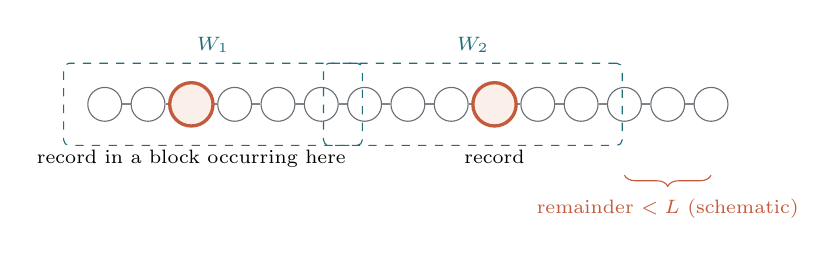
\begin{tikzpicture}[
  pt/.style={circle,draw=ink!65,fill=white,minimum size=4.3mm,inner sep=0pt},
  sel/.style={circle,draw=accenttwo,very thick,fill=softorange,
             minimum size=5.5mm,inner sep=0pt},
  path/.style={thick,ink!55},
  win/.style={draw=accent,rounded corners=2pt,dashed,inner sep=3mm},
  lab/.style={font=\scriptsize,accent}
]
\foreach \x in {0,...,14}{
  \node[pt] (v\x) at (.55*\x,0) {};
}
\foreach \x [evaluate=\x as \y using int(\x+1)] in {0,...,13}{
  \draw[path] (v\x)--(v\y);
}
\node[sel] at (v2) {};
\node[sel] at (v9) {};
\node[win,fit=(v0)(v5),label={[lab]above:$W_1$}] {};
\node[win,fit=(v6)(v11),label={[lab]above:$W_2$}] {};
\node[font=\scriptsize,anchor=north] at ($(v2)+(0,-.45)$)
  {record in a block occurring here};
\node[font=\scriptsize,anchor=north] at ($(v9)+(0,-.45)$) {record};
\draw[decorate,decoration={brace,mirror,amplitude=4pt},accenttwo]
  ($(v12)+(0,-.9)$)--($(v14)+(0,-.9)$)
  node[midway,below=5pt,font=\scriptsize] {remainder $<L$ (schematic)};
\end{tikzpicture}
\caption{Record placement on a long virtual path (drawn with small schematic
windows).  Hall's theorem chooses the host block inside each window.  The
decoder does not reconstruct the windows; it searches for a named record.}
\label{fig:windows}
\end{figure}

For a virtual edge $f$ and virtual vertex $z$, define
$\dist_H(f,z)$ as the minimum distance from $z$ to an endpoint of $f$.

\begin{lemma}[Record coverage]
\label{lem:record-coverage}
Every edge of a long component of $H$ is at distance less than $2L$ from a
selected virtual copy carrying a record.
\end{lemma}

\begin{proof}
Within a full window, every edge is fewer than $L$ steps from that window's
selected copy.  The same is true at a boundary between consecutive full
windows using a selected copy from one of the two adjacent windows.

For a path, only a terminal remainder exists.  From the selected copy in the
last full window to the end of the remainder is fewer than $2L$ steps.  For a
cycle, the remainder lies on the wraparound arc between the last and first
full windows.  Every edge on that arc is fewer than $2L$ steps from the
selected copy in at least one of those two windows.  When $N=L$, the one
window covers all vertices; the closing cycle edge is also fewer than $L$
steps from its selected copy.  These cases include singleton path endpoints
and an empty remainder.
\end{proof}

\subsection{The residual-orientation rule}
\label{sec:orientation-rule}

We can now define the decoder's orientation of a queried residual edge
$f$ in the parsed virtual graph $\widehat H$.  The parser constructing
$\widehat H$ from a standalone finite view is specified in
\cref{sec:decoder}; the present rule is applied only to that graph, not to
an unavailable ambient component.  Its paths, distances, and connected
components in the following three steps are all computed in $\widehat H$.
The view is rooted at the original query edge $e$.  Put
\[
 \rho_{\rm host}=\eta+(2L+1)(2\eta+1).                       \tag{7.4}
\]
A parsed record is \emph{host-safe} if its named copy's physical host center
has distance at most $\rho_{\rm host}$ from $e$ in the supplied physical
view graph.  Of the two block incidences of a residual edge $f$, take the
one at the lower center key (using the same malformed-input tie-break as
elsewhere); let $a(f)$ be the virtual copy containing that incidence.  This is
the canonical anchor of $f$.
\begin{enumerate}[label=\textbf{\arabic*.},leftmargin=2.3em]
\item Compute the connected component of $f$ in the finite standalone parsed
      virtual graph.  If its vertex count is below $L$, use the canonical
      short-component direction.
\item Otherwise enumerate the records of all valid parsed cells.
      First treat every non-host-safe record as empty.  Only
      after this safety filter is a remaining record eligible: its
      \emph{named copy} $(B,j)$ must lie in the same $\widehat H$-component and satisfy
      $\dist_{\widehat H}((B,j),a(f))\le2L+1$.  Thus a slot stored at $B$ but naming a
      different copy of $B$ on another strand or outside this interval is
      ignored.  Choose the eligible semantic record with least lexicographic
      key
      \[
       ((\id(z_B),\text{visible-vertex tie-break}),j,
          \text{direction bit}),
      \]
      read the absolute direction of its reference incidence, and propagate
      the unique consistent direction to $f$.  Slot provenance has already
      been discarded; equal semantic records from several slots are one
      candidate.
\item If there is no eligible record, use the same canonical coherent
      component orientation as in the short case: the component's least
      residual edge points from its lower-key to its higher-key virtual
      endpoint, and this direction is propagated to $f$.
\end{enumerate}
Invalid record values are empty.  Duplicate or disagreeing records are
resolved by the least-key rule.  In particular, a syntactically valid record
at an unsafe outer-boundary host is empty \emph{before} component membership,
distance, or minimum-key selection is considered.  Thus this prescription
gives one absolute direction to every residual edge on every parsed labeling,
even a malformed one.

Correctness for the interior incidences needed by an original query is proved
in \cref{lem:orientation-correct}, after establishing exact reconstruction
from the available physical ball.  The encoder itself uses its chosen
global strand directions and does not run this parser.

The distinction between a physical block and a named virtual copy is
essential: one block can occur several times in $H$.  The explicit filter in
step 2 is what makes repeated occurrences harmless.

\begin{example}[Why a record names a copy]
Suppose one physical block $B$ has copies $(B,1)$ and $(B,2)$ on two different
virtual strands.  A slot physically stored in $B$ may name $(B,2)$ and record
the direction of its reference incidence.  A query on the strand through
$(B,1)$ may still encounter the physical block $B$, but that record carries
no orientation information about $(B,1)$ and is ignored.  A query near
$(B,2)$ accepts it.  Merely naming the host block would conflate the two
strands and could destroy the balance guarantee.
\end{example}

\section{The encoder}
\label{sec:encoder}

We now encode an arbitrary target vector $x\in\bits^{E(G)}$.  Operations are
performed independently in each connected component.

\subsection{Large components}

For a component with at least $b_\star$ vertices, the encoder performs the
following finite operations.
\begin{enumerate}[leftmargin=2.1em]
\item Choose a maximal separated center set, form its Voronoi blocks, and
      construct each canonical buddy matching.
\item Construct $J$, cancel parallel pairs to obtain $K$, split incidences
      to obtain $H$, form the long-component windows, and choose a Hall
      assignment from \cref{lem:window-allocation}.
\item Orient the short strands canonically and the long strands in their
      positive indexed direction.  Write their records into the assigned
      slots; fill unused slots with the empty value.
\item Restore the canceled quotient pairs and give every edge the owner from
      \cref{lem:ownership}.  Sort the edges owned by $B$ by $\kappa$, write
      their target bits into its $\pi_B$ payload fields, and pad unused
      fields with zero.
\item Assemble the logical integer $W_B$ and apply the explicit unranking map
      following (6.9).  Put the resulting symbols on $F_B$, with the fixed
      center star on $N[z_B]$.
\end{enumerate}
The ownership lemma shows that every target coordinate fits, while
\cref{lem:slot-capacity} shows that every logical block word has a physical
realization.  Every edge is written exactly once.

All choices can, if desired, be made canonical by taking the lexicographically
first maximal center set and Hall assignment.  Their computational cost is
irrelevant: the model restricts the decoder, not the encoder.

\subsection{Small components}
\label{sec:small}

Let a component have $n<b_\star$ vertices.  Every vertex can see the entire
component within radius $b_\star-1$.  Order its vertices by identifier and
its edges by $\kappa$, writing them as $v_0,\ldots,v_{n-1}$ and
$e_0,\ldots,e_{m-1}$.  Encode the integer
$T=\sum_{j=0}^{m-1}x_{e_j}2^j$ by its $n$ base-$\alpha$ digits:
$\ell(v_i)=\floor{T/\alpha^i}\bmod\alpha$.  This fits because
\[
                         \frac{dn}{2}\le s_d n.                 \tag{8.1}
\]
The inverse forms $Z=\sum_i\ell(v_i)\alpha^i$ and, if $Z<2^m$, reads
the bit $\floor{Z/2^j}\bmod2$ at edge $e_j$; otherwise it returns zero.
On an arbitrary standalone view with $k<b_\star$ visible vertices, use
these same formulas on the whole visible induced graph.  If IDs repeat,
use the total orders specified in \cref{sec:decoder}.  No inequality between
the raw graph's edge count and $s_dk$ is needed to define this decoder.
The hybrid
decoder selects this branch solely by the label-independent inequality
$k<b_\star$; it does not test boundary stubs or closedness.  On a genuine
extracted view the advertised radius makes this exact.  If the queried
component has fewer than $b_\star$ vertices, the whole component is visible
and $k=n$.  If it has at least $b_\star$ vertices, connectedness implies that
the radius-$(b_\star-1)$ ball from a root endpoint already contains at least
$b_\star$ vertices (or the whole component), so $k\ge b_\star$.  Thus
accidental star patterns in a genuine small-component word cannot affect
parsing.

\section{A total local decoder}
\label{sec:decoder}

A decoding function must be defined not only on codewords, but on every
raw finite view.  All five stages below operate solely on the supplied
finite graph, labels, and local indices.  We then prove in
\cref{sec:locality} that an extracted radius-$R_d$ view contains enough
information for these operations to recover its root target.

A malformed raw view may repeat numerical IDs.  To keep every parsed choice
total, append the canonical visible local vertex index to every vertex-ID
key.  Thus the parsed assignment key is
$(\dist(v,c),\id(c),\operatorname{loc}(c))$, and the parsed edge key is its
unordered endpoint-ID pair followed by the unordered local-endpoint pair.
Pairs here are listed in increasing order and compared lexicographically.
All distances in the parser are distances in the supplied induced graph,
with distance $+\infty$ between its different connected components.
These last coordinates are deterministic tie-breaks only: on a genuine
extracted view the IDs are injective, so the orders reduce to the encoder's
ID and $\kappa$ orders.  The record key in \cref{sec:orientation-rule} uses
the same parsed-center convention.

The decoder has the following five stages.
\begin{enumerate}[label=\textbf{\arabic*.},leftmargin=2.3em]
\item \textbf{Select the component branch.}
      Let $k$ be the total number of visible vertices.  If $k<b_\star$,
      regard the whole visible induced graph and its labels as one finite
      codeword, apply the rank/unrank decoder of \cref{sec:small}, and return
      its queried-edge bit (or zero when the label rank is outside the target
      interval).  Otherwise enter the parsed large-component branch.

\item \textbf{Parse stars and cells.}
      On the large branch, call a visible vertex a parsed marked center when
      its label is $1$ and every one of its neighbors in the visible induced
      graph has label $0$; opaque outside port stubs are not inspected.  Define
      \[
       \gamma(v)=\arg\min\{(\dist(v,c),\id(c),\operatorname{loc}(c)):
          c\text{ marked and }\dist(v,c)\le\eta\},             \tag{9.1}
      \]
      and put $\gamma(v)=\bot$ if the set is empty.  For a marked center $c$,
      let $\widehat B_c=\{v:\gamma(v)=c\}$.  Its members lie within parsed
      distance $\eta$ of $c$, but an arbitrary raw view has no degree bound,
      so a separate size guard is essential.  Call the cell \emph{valid} iff
      it contains $c$ and every visible neighbor of $c$, its induced graph is
      connected,
      \[
                  b_\star\le |\widehat B_c|\le B_{\max},
      \]
      and $c$ has exactly $d$ visible neighbors.  For each valid cell set
      $B:=\widehat B_c$ and construct its buddy matching and the
      quotient-independent quantities $N_B$, $c_B$, $\pi_B$, and $\sigma_B$.
      Invalid cells expose the all-zero logical word and no nonempty record.
      The size and degree guards are automatic for completely reconstructed
      genuine encoder cells, not for arbitrary raw views.
      For a valid cell, $b\ge b_\star$ and the center's $d$ neighbors ensure
      $b-d-1\ge0$; the arithmetic proof of \cref{lem:surplus} gives
      $\sigma_B\ge0$ even if other raw vertices have excessive degree.

\item \textbf{Build the quotient and decode fields.}
      Construct the parsed quotient on all marked centers.  An original edge
      with a $\bot$ endpoint is omitted; an edge whose endpoints map to the
      same marked center is internal; every other edge becomes a quotient
      edge.  Parallel cancellation and incidence splitting include
      invalid marked cells, but such cells contribute no records.  The
      residual degree now determines $\nu_B$, $w_B$, $t_B$, and $\ell_B$ for each
      valid cell.  Rank its physical data word.  If the word is illegal or
      its rank is outside the image in (6.9), set its entire logical word to
      zero; the parser retains no separate invalid-word flag.
      The parsed residual quotient is simple even on malformed inputs.
      Consequently its incidence splitting always produces paths and cycles
      of degrees one and two, so every orientation operation in the next
      stage is defined.

\item \textbf{Recover directions.}
      Apply the total residual-orientation rule of
      \cref{sec:orientation-rule}.  In particular, discard every record whose
      host is outside the radius-$\rho_{\rm host}$ inner edge ball before the
      component/distance filter and least-record selection.  Keep the fixed
      opposite directions on canceled pairs.

\item \textbf{Find the owner and read payload.}
      For a queried original edge $e$, return zero immediately if an endpoint
      maps to $\bot$ or if either relevant parsed cell is invalid.  Otherwise,
      internal ownership or the parsed quotient direction determines an
      eventual owner $B$.  Enumerate by the parsed edge key above all internal
      edges of $B$ and all parsed quotient edges directed out of $B$, omitting
      $\bot$-endpoint edges exactly as in the quotient.  If this list has more
      than $\pi_B$ entries, return zero.  Otherwise return the payload
      coordinate at the rank of $e$ in this list.  A malformed physical word
      has already become the all-zero logical word at Stage 3.
\end{enumerate}

These conventions also cover missing records, excess records, disagreeing
records, unsafe boundary-host records, extra stars, disconnected parsed
cells, and owner overload.  On a
malformed labeling, separately decoded residual edges need not form a
balanced orientation, but every edge receives a deterministic absolute
direction, and the overload guard prevents an out-of-range payload access.
Thus the decoder is total.

There is no circularity in the definition: star patterns determine cells;
cells and the visible graph determine buddy matchings, the quotient, and
field lengths; the finite code reveals records; records determine ownership;
only then is the payload interpreted.  We prove exact recovery next.

\section{Correctness, locality, and the explicit radius}
\label{sec:locality}

Fix a genuine encoded view $X=\mathsf{View}_{R_d}(G,\id,\ell,e)$ whose
root lies in a large component.  We identify its local vertices with the
corresponding ambient vertices using their distinct IDs.  Put
\[
 g=2\eta+2,\qquad \zeta=2\eta+1.                                  \tag{10.1}
\]
If two global blocks are adjacent in the quotient, their centers
have graph distance at most $\zeta$: follow a path of length at most $\eta$
from the first center to a witnessing boundary endpoint, cross that edge,
and follow at most $\eta$ further edges to the second center.  The same
estimate holds for parsed cells, with distances in $X$, because (9.1)
assigns a vertex only to a center within distance $\eta$.  Thus
\[
 \text{one global or parsed virtual step moves its host center
 by at most }\zeta.                                               \tag{10.2}
\]
This bound is valid even when successive virtual copies have hosts already
visited by the walk.

Recall $\rho_{\rm host}=\eta+(2L+1)\zeta$.  The needed physical radius is
\[
 r_{\rm lit}=\rho_{\rm host}+g
   =\eta+(2L+1)(2\eta+1)+(2\eta+2).                            \tag{10.3}
\]
Direct expansion gives
\[
 R_d-r_{\rm lit}=\eta+2L+3>0.                                 \tag{10.4}
\]
In particular, every radius-$g$ neighborhood of a vertex within distance
$\rho_{\rm host}$ of $e$ is wholly present in $X$.

We will repeatedly use two elementary facts about induced balls.  Distance
to the root edge is unchanged by extraction: a shortest path to an endpoint
of $e$ stays in the edge ball.  More generally, if
$\dist_G(e,c)+u\le R_d$, every ambient path of length at most $u$ starting
at $c$ lies in $X$.  Consequently its radius-$u$ neighborhood, including
all distances at most $u$ from $c$, is reproduced exactly.  These facts
follow directly from the triangle inequality and the definition of
$V_{R_d}(G,e)$.

\begin{lemma}[Exact reconstruction at an interior center]
\label{lem:interior-reconstruction}
A parsed marked center $c$ with $\dist_X(e,c)\le\rho_{\rm host}$ is a
genuine encoder center.  Conversely, every encoder center satisfying this
distance bound is parsed as marked.  At each such center the following
data are exact:
\begin{enumerate}[label=\textup{(\roman*)}]
\item its entire cell $B_c$, its internal edges, and its buddy matching;
\item every boundary edge of $B_c$ and the assigned center of its outside
      endpoint;
\item its residual quotient incidences, their order, their pairing,
      the local copy indices, and the reference incidence at each copy;
\item its logical field lengths, its payload, and every stored record.
\end{enumerate}
In particular its parsed cell is valid.  If a residual edge joins two
such interior centers, its two virtual endpoints agree with the global
ones.
\end{lemma}

\begin{proof}
All neighbors of $c$ are visible, so its parsed star test is the global
star test.  By \cref{lem:star-code}, that test identifies precisely the
encoder centers.

Every vertex that could belong to $B_c$ is within distance $\eta$ of $c$,
by \cref{lem:block-geometry}.  To decide the assignment of any such
vertex $v$, it suffices to inspect centers within distance $\eta$ of $v$.
All these potential centers are within $2\eta$ of $c$, and all their
neighbors are within $2\eta+1$.  Their stars, the distances relevant to
the assignment, and the ID comparisons are therefore exact.  No spurious
boundary star can compete in this assignment.  Moreover a parsed member
of $\widehat B_c$ must itself be within $\eta$ of $c$, so there are no
additional parsed members outside this candidate region.  Hence
$\widehat B_c=B_c$.  The induced cell graph and its ordered greedy matching
are then identical.  The global cell geometry and regularity imply all
the validity guards.

All endpoints of edges incident with $B_c$ are within $\eta+1$ of $c$.
Their assignments require at most another $\eta+1$ hops, hence lie in
the available radius $g=2\eta+2$ neighborhood.  This proves (ii), including
the absence of $\bot$ endpoints.  Every parallel quotient edge incident
with $B_c$ is among these edges.  Thus the complete parallel lists,
their cancellations, the remaining neighbor-center keys, and all incidence
pairings at $B_c$ are exact.  This proves (iii).  Notice that this argument
needs the center assigned to a neighboring boundary endpoint, not a
reconstruction of that neighbor's entire cell.

The cell size, center degree, matching, residual degree, physical labels,
and their orders now coincide.  Therefore the code rank, the field lengths
in (4.10) and (6.1), and all decoded fields coincide as well.  The encoder's
rank lies in the reserved interval, so the zero fallback does not apply.
This proves (iv).  At two interior endpoint centers, (iii) identifies both
copy indices of a residual edge, proving the last assertion.
\end{proof}

\begin{lemma}[Comparison of bounded virtual walks]
\label{lem:virtual-walks}
Let $B$ be an encoder block whose center is within distance $\eta$ of
$e$, and let $z$ be any virtual copy above $B$.
Every global or parsed virtual walk of length at most $2L+1$ starting at
$z$ has the same sequence of named copies and residual edges in the other
graph.  The same assertion holds for a parsed walk of length $2L+2$
if its terminal host is host-safe.
\end{lemma}

\begin{proof}
By (10.2), the host center of the vertex at step $i$ is within distance
$\eta+i\zeta$ of $e$, in the appropriate physical graph.  For
$i\le2L+1$ this is at most $\rho_{\rm host}$.  Thus all these hosts
satisfy \cref{lem:interior-reconstruction}.  Starting with the exact local
copy at $B$, its residual edge and the local index of the next copy are
identical whenever both endpoint hosts are interior.  Induction on the
walk length proves the assertion in either direction.  For the extra
terminal step all earlier hosts are interior by the same bound, and
the terminal host is interior by its explicit safety hypothesis.  Apply
the last assertion of \cref{lem:interior-reconstruction} to that step.
\end{proof}

\begin{lemma}[The short-component test is correct near the query]
\label{lem:short-test}
Under the hypotheses of \cref{lem:virtual-walks}, if the global component
of $z$ has fewer than $L$ vertices, its entire parsed component is the
same component.  If the global component has at least $L$ vertices,
the parsed component has at least $L$ vertices.
\end{lemma}

\begin{proof}
In the first case every vertex of the global component is reached from
$z$ by a path of length at most $L-2$.  All these vertices and edges are
reconstructed by \cref{lem:virtual-walks}.  A parsed edge leaving this
set would extend such a path by one step, still well within $2L+1$;
the same lemma would give a global edge leaving the global component,
a contradiction.  Therefore there are no extra parsed vertices.

For the second case, a connected graph with at least $L$ vertices has
at least $L$ vertices within distance $L-1$ of any fixed vertex: either
this ball is the whole component, or a shortest path to a vertex outside
it already contains $L$ vertices inside it.  Choose $L$ distinct such
vertices and paths to them.  The walk lemma embeds these paths into the
parsed graph.  The named-copy correspondence is injective, since a center
ID and its local copy index uniquely identify a vertex.  Hence the parsed
component contains at least $L$ vertices.
\end{proof}

\begin{lemma}[Correctness of recorded orientations]
\label{lem:orientation-correct}
Let $B$ be an encoder block whose center is within distance $\eta$ of
the original root edge $e$.  For every residual edge incident with $B$,
the rule of \cref{sec:orientation-rule}, run in $X$, returns the encoder's
direction of that edge.
\end{lemma}

\begin{proof}
Let $f$ be such a residual edge and let $z$ be its virtual endpoint above
$B$.  The other host center is at most one quotient step away, so both
virtual endpoints of $f$ are exact.  If the global component is short,
\cref{lem:short-test} identifies its whole parsed component.  The
canonical edge order and the endpoint keys agree, so its canonical
orientation agrees.

Suppose the global component is long.  The same lemma says the parsed
component has at least $L$ vertices, so the decoder takes its record
branch.  We prove both that every retained candidate is correct and
that a candidate exists.

For a retained candidate, take a parsed walk of length at most $2L+1$
from the anchor $a(f)$ to its named copy.  Prepend $f$ if needed to
start at $z$.  The resulting walk has length at most $2L+2$, and its
terminal host is safe by the record filter.  By
\cref{lem:virtual-walks}, it is a global walk with the same named copies.
By \cref{lem:interior-reconstruction}, the terminal record is the exact
readback of an encoder slot, including its reference incidence and
direction bit.  Every nonempty encoder slot describes the chosen
orientation of its named copy's global component.  The global walk shows
that this is the component containing $f$.  Propagating that direction
back along the walk therefore gives the encoder's direction of $f$.

Conversely, \cref{lem:record-coverage} supplies a recorded copy at distance
less than $2L$ from one endpoint of the global edge $f$.  Since distances
are integral, it can be reached from $z$ in at most $2L$ steps, including
a possible initial traversal of $f$.  Every host on that walk is interior;
the walk and the record are reconstructed exactly by
\cref{lem:virtual-walks,lem:interior-reconstruction}.  Its host is safe.
In the parsed graph the anchor $a(f)$ is at most one step from $z$,
so the record is within $2L+1$ of that anchor and is eligible.  Thus the
candidate set is nonempty, all its elements describe the same global
direction, and its least element gives the correct direction.
\end{proof}

\begin{lemma}[Exact recovery]
\label{lem:exact-recovery}
On every labeling produced by the encoder, the radius-$R_d$ decoder
returns $x_e$ at every original edge $e$.
\end{lemma}

\begin{proof}
The visible-count branch is correct by \cref{sec:small}, since
$R_d\ge b_\star-1$.  On a small component, base-$\alpha$ encoding and
binary digit extraction are inverse.

Now let $e$ lie in a large component.  Each block containing an endpoint
of $e$ has its center within distance $\eta$ of $e$.  Its cell, validity
guards, and incident quotient data are exact by
\cref{lem:interior-reconstruction}.  If $e$ is internal, its owner is
therefore the correct common block.  If $e$ is in a canceled parallel
pair, the identical edge list and center order give its correct
direction.  Otherwise \cref{lem:orientation-correct} gives its correct
residual direction.  In all cases the decoder chooses the encoder's owner,
say $B$.

We must also recover the position of $e$ in $B$'s payload, not just its
owner.  The reconstruction lemma supplies every internal and boundary
edge of $B$ with the correct outside assignment.  Canceled directions
agree, and \cref{lem:orientation-correct} applies separately to every
residual incidence of $B$.  Thus the entire parsed list of edges owned
by $B$ equals its global list, including its order by $\kappa$.
No incident edge is omitted for a $\bot$ endpoint.  By
\cref{lem:ownership} the list has at most $\pi_B$ elements, so the
overload guard is inactive.  Finally the logical word is read back exactly,
and its payload coordinate for $e$ is precisely the stored bit $x_e$.
\end{proof}

Every operation of the decoder is a finite computation on the supplied
raw view, including on malformed input.  The proof uses exact ambient
reconstruction only at the interior centers specified above; it makes
no claim that an arbitrary cell at the outer boundary is genuine.
Because the input is just the radius-$R_d$ view, the reconstruction and
recovery lemmas establish the advertised locality.  For fixed $d$,
genuine views have bounded size, while arbitrary raw structures may have
larger size.  The parser still terminates on every finite raw structure.
No bound on its computational running time is part of the theorem.

The radius is polynomial in $d$.  For $d\ge3$,
\[
 B_{\max}\le3(d-1)^\eta,\qquad
 \chi_d=O(\eta\log d)=O(d^2\log d).
\]
Indeed $d/(d-2)\le3$ gives the first inequality from (2.4);
the second follows by taking logarithms and using
$\eta=128(d+1)^2-2$.  Hence $L=O(d^3\log d)$ and
\[
 R_d=O(d^5\log d).                                            \tag{10.5}
\]
For cubic graphs,
\begin{align*}
 b_\star&=1024,& \eta&=2046,&
 B_{\max}&=3\cdot2^{2046}-2,\\
 \chi_3&=2050,& L&=123000,&
 R_3&=246003\cdot4094=1{,}007{,}136{,}282.                     \tag{10.6}
\end{align*}
Here $2^{2049}<3B_{\max}<2^{2050}$ verifies the logarithm ceiling
without numerical approximation.  These constants are sufficient, not
claimed to minimize the radius.

\section{Order normalization and reversible strip maps}
\label{sec:normalization}

We turn to the lower bound in even degree.  At the putative rate $d/2$,
vertex labels and edge targets have exactly the same cardinality on every
$d$-regular graph.  Hence surjectivity would make every finite global decoder
map bijective.  The argument below converts these finite bijections into a
reversible map on a one-dimensional strip.

The decoder may initially use the numerical values of IDs, whereas reflection
only respects their order.  The following exact normalization removes this
issue.  It is a direct Ramsey argument specialized to our surjectivity model.

\begin{lemma}[Order normalization]
\label{lem:order-normalization}
Fix $d,r$ and a finite alphabet.  Suppose a radius-$r$ decoder is surjective
on every finite simple $d$-regular graph for every injective natural-number
ID assignment.  There is a decoder of the same radius and alphabet which is
still surjective on that family and depends on IDs only through their relative
order in the queried view.
\end{lemma}

\begin{proof}
One may take $q=2\sum_{i=0}^r d^i$ as a bound on the number of visible
vertices: at most $d^i$ walks of length $i$ start at either endpoint.
For each $1\le j\le q$, combine into one finite color the original decoder's
complete truth table on every $j$-vertex rooted topology of maximum degree
at most $d$, every port template with $d$ entries at each vertex, and every
physical-label assignment when a given $j$-set of IDs is placed increasingly
on the ordered template positions.  There are finitely many templates and
labels, so the color set is finite.

We recall the short proof of the finite-color infinite Ramsey theorem.  It is
by induction on the subset size.  The singleton case is infinite pigeonhole.
For the step from $j$ to $j+1$, recursively choose points $z_i$ and nested
infinite tails so that, after fixing $z_i$, the color is constant on all
$j$-subsets of the next tail; this uses the induction hypothesis.  Infinitely
many $z_i$ have the same resulting color.  Any $j+1$ of those points has the
color attached to its least point, so they form an infinite homogeneous set.

Apply this theorem successively for $j=1,\ldots,q$, restricting the current
infinite set after each application.  We obtain one infinite ID set $I$
homogeneous for every relevant view size.  On a determining view
of size at most $q$ with a strict ID order, define the new decoder to be the
common truth-table value obtained from increasing IDs in $I$; on every other
raw view give it an arbitrary fixed output, so it remains total.  For a finite
instance, relabel the vertices order-preservingly into $I$.  The given decoder
has a valid encoding there.  Copy its physical labels back.  Homogeneity
preserves every local truth-table value, and the order-preserving relabeling
also preserves neighbor-ID ports.  Thus the new decoder realizes the original
target.  The normalized rule ignores numerical magnitudes; the canonical
view enumeration and ports still retain the relative order.
\end{proof}

Fix an even degree $d=2k$, $k\ge1$, and assume for contradiction that a
$k$-bit decoder is surjective on all finite simple $2k$-regular graphs.  By
\cref{lem:order-normalization}, assume it is order-invariant.  Choose the
positive jump lengths
\[
 a_1=1,\qquad a_j=2(j-1)\quad(2\le j\le k),
 \qquad S_k=\sum_{j=1}^k a_j=1+k(k-1).                      \tag{11.1}
\]
Thus $S_k$ is odd.  Put $M=\max_j a_j$, taking $M=1$ for $k=1$.  For
$n>2M$, define
\[
 G_n=\operatorname{Cay}\bigl(\mathbb Z/n\mathbb Z,
                    \{\pm a_1,\ldots,\pm a_k\}\bigr),
 \qquad e_{j,i}=\{i,i+a_j\}.                               \tag{11.2}
\]
The graph is connected because $a_1=1$.  It is simple and $2k$-regular:
the positive jumps are distinct and less than $n/2$, so none is zero, no two
are congruent up to sign, and reversing a named edge cannot name it again.
Consequently (11.2) names every edge exactly once.

For every total order $\prec$ on $G_n$, the decoder induces
\[
 D_{n,\prec}:(\bits^k)^{\mathbb Z/n\mathbb Z}
     \longrightarrow\bits^{E(G_n)}.                        \tag{11.3}
\]
Both sides have $2^{kn}$ elements.  Surjectivity therefore makes
$D_{n,\prec}$ a bijection.  A finite total order is realized by assigning
its positions the distinct natural IDs $0,\ldots,n-1$.

A \emph{configuration} over a finite alphabet $C$ is a function
$x:\mathbb Z\to C$; the space $C^{\mathbb Z}$ of all such configurations
is called the \emph{full shift}.  A map $F:C^{\mathbb Z}\to C^{\mathbb Z}$ has
dependence radius $m$ if $F(x)_i=F(x')_i$ whenever $x,x'$ agree on
$[i-m,i+m]$.  Its coordinate rule may depend on $i$.  We call it
\emph{$N$-periodic} when it commutes with translation by $N$ sites,
equivalently when the coordinate rules repeat every $N$ sites.

The order-normalized decoder can be applied to the infinite jump graph
with any total order: each finite view is evaluated by its relative order,
or equivalently by replacing its visible IDs with their ranks.
No order-preserving assignment of natural IDs to the whole infinite graph
is required.  Write
\[
                         m=(r+2)M.
\]
The edge $e_{j,i}$ has its endpoints in $[i,i+M]$.
Its radius-$r$ vertex view, together with the additional neighbor layer
needed to determine all its ports, is contained in $[i-m,i+m]$.
Thus grouping the $k$ output bits based at $i$ gives a map of dependence
radius at most $m$ for every fixed total order.

\begin{lemma}[Realizing a finite fragment on a ring]
\label{lem:finite-fragment}
Fix any total order of the infinite jump graph and a finite interval
$J=[u,v]\subseteq\mathbb Z$.  For a sufficiently large $n>2M$, one can order
$G_n$ so that all decoder outputs based in $J$ agree with the infinite
ordered graph, for every assignment of labels on $[u-m,v+m]$
copied to the corresponding ring vertices.
\end{lemma}

\begin{proof}
Choose $n>2(v-u+2m+2M+1)$.  Projection modulo $n$ is injective on
$I=[u-m,v+m]$.  For two coordinates in $I$, a difference congruent to a
jump $\pm a_j$ modulo $n$ must equal that jump as an integer: the size of
$n$ excludes an additional nonzero multiple of $n$.  Hence projection
preserves the induced edges on $I$.  A walk of at most $r+1$ jumps
starting at an endpoint of $e_{j,i}$, $i\in J$, stays in $I$.
All determining views and their neighbor layers are therefore reproduced,
with no additional vertices or shortcuts from wrapping around the ring.
Impose the given order on the projected vertices of $I$ and extend it
arbitrarily to the other ring vertices.  Local order comparisons and
neighbor-ID port positions are identical.  Since labels outside $I$
are not read by these queries, all the specified outputs agree.
\end{proof}

\begin{lemma}[Finite-alphabet compactness and inverse coordinates]
\label{lem:configuration-compactness}
Let $C$ be a finite nonempty alphabet and let
$F:C^{\mathbb Z}\to C^{\mathbb Z}$ have finite dependence radius.
Every sequence of configurations has a subsequence that eventually
stabilizes at each coordinate.  The image of $F$ is closed under these
coordinatewise limits.  In particular, if every finite interval of every
desired output can be realized, $F$ is onto.
If $F$ is bijective, then for each $i$ there is a finite $t_i$ such that
$F^{-1}(y)_i$ is determined by $y|_{[i-t_i,i+t_i]}$.
\end{lemma}

\begin{proof}
List the coordinates as $0,1,-1,2,-2,\ldots$.  Repeatedly pass to an
infinite subsequence constant at the next coordinate, using finiteness of
$C$.  The diagonal subsequence stabilizes at every coordinate.
A finite-radius map preserves this convergence because each output
coordinate reads only finitely many input coordinates.

If $F(x^{(n)})$ converges coordinatewise to $y$, extract a convergent
subsequence of the inputs with limit $x$.  Then $F(x)=y$, proving
closedness.  If every interval $[-n,n]$ of $y$ has a preimage, choose
one such input for each $n$ and apply the same argument; the image limits
to $y$, proving surjectivity.

Finally suppose no $t_i$ works for a fixed $i$.  For each $n$ choose
outputs $y^{(n)},z^{(n)}$ agreeing on $[i-n,i+n]$ whose preimages differ
at $i$.  Apply the diagonal argument to the pairs of preimages, over
the finite alphabet $C\times C$.  Their limits $x,x'$ still differ
at $i$, since the pair of symbols at $i$ eventually stabilizes.
For each output coordinate $j$, finite dependence and the growing
agreement intervals give $F(x)_j=F(x')_j$.  This contradicts injectivity.
\end{proof}

\begin{lemma}[Periodic finite bijections give a reversible map]
\label{lem:periodic-reversible}
Let $C$ be a finite nonempty alphabet, let $N\ge1$, and let
$F:C^{\mathbb Z}\to C^{\mathbb Z}$ have a finite dependence radius and an
$N$-periodic local rule.  If $F$ restricts to a bijection on the
configurations whose period divides $tN$ for every $t\ge1$, then $F$
is bijective and $F^{-1}$ has a uniform finite dependence radius.
\end{lemma}

\begin{proof}
Any prescribed output word on a finite interval extends to a
$tN$-periodic configuration for a sufficiently large $t$.  The assumed
bijection supplies a same-period preimage.  Thus
\cref{lem:configuration-compactness} makes $F$ onto.

For injectivity, group consecutive $N$ sites into single symbols of
$A=C^N$.  The blocked map has a translation-invariant finite local rule;
choose a radius $r_0\ge1$ for that rule.  A pair of blocked input
configurations has equal outputs precisely when each pair window of
length $2r_0+1$ gives equal central outputs.  This condition has the
following explicit finite graph representation.  Its vertices are all
allowed length-$(2r_0+1)$ words over $A\times A$, and a directed edge
joins two such words when their last and first $2r_0$ entries agree.
Bi-infinite walks give exactly the equal-output pairs, by reading
the central entries of successive windows.

Suppose two distinct infinite inputs have equal outputs.  If they differ
at infinitely many blocked coordinates, there are infinitely many window
vertices with unequal central entries.  Some such vertex occurs at
two different positions, because the graph is finite.  Repeating the
directed segment between these positions produces a periodic walk
with an unequal central entry.  Reading its centers gives two distinct
periodic inputs with equal outputs.  Their unblocked period is a multiple
of $N$, contradicting one of the finite-period bijections.

Otherwise the difference is contained in a finite blocked interval
$[a,b]$.  Choose $t>b-a+4r_0+1$.  On a ring of $t$ blocks, copy both
inputs on $[a-2r_0,b+2r_0]$ and give them a common fixed symbol
elsewhere.  Their difference is still nonempty and is confined to
$[a,b]$.  Every output window meeting this difference is contained
in the copied interval and has the equal outputs of the original
collision.  All other output windows see identical inputs.  Equivalently,
periodically repeating the two ring words gives a collision of period
$tN$, again impossible.

Thus $F$ is bijective.  By \cref{lem:configuration-compactness}, each
inverse coordinate has a finite dependence interval.  The inverse
commutes with translation by $N$, because $F$ does.  Take the maximum
of the dependence radii at the $N$ representatives $0,\ldots,N-1$;
translation then gives the same finite bound at every coordinate.
\end{proof}

Choose $N>4(r+2)M$.  Projection modulo $N$ is then injective on every
determining view in the infinite jump graph, including the neighbor layer
which fixes boundary ports.  Fix any ranking $\pi$ of the residues modulo
$N$.  On $\mathbb Z$, order $i=u+tN$, $0\le u<N$, lexicographically by
$(\pi(u),t)$.  No determining view contains two positions with the same
residue, so its comparison pattern is $N$-periodic.

On $G_{tN}$, use the finite keys $(\pi(u),v)$, $0\le v<t$, and replace them
by their ranks.  Every local comparison is decided by the distinct primary
residue ranks, including at the global wrap.  Hence topology, order, and
ID-induced ports are exactly the finite projection of the infinite
environment.

Group the $k$ edge outputs based at $i$ into one $k$-bit output cell:
\[
 P(x)_i=\bigl(D(x)_{e_{1,i}},\ldots,D(x)_{e_{k,i}}\bigr).
                                                                    \tag{11.4}
\]
This is an $N$-periodic finite-radius map on the $2^k$-symbol full shift.
On configurations whose period divides $tN$, it is precisely the bijection
(11.3).  Therefore \cref{lem:periodic-reversible} makes $P$ bijective with
a uniform finite-radius inverse.  Grouping every $N$ consecutive sites
into one cell gives a reversible one-dimensional cellular automaton.

\section{A self-contained rational flow index}
\label{sec:index}

We prove the one-dimensional index facts needed below by counting finite
input/output interfaces.  For historical context on reversible cellular
automata and their information-flow invariants, see
Hedlund~\cite{Hedlund1969ShiftDynamical},
Kari~\cite{Kari1996BlockPermutations}, and
Gross, Nesme, Vogts, and Werner~\cite{GrossNesmeVogtsWerner2012Index}.
The argument here requires none of their results.

Call a map \emph{reversible and local} if it is a bijection and both it
and its inverse have a uniform finite dependence radius.  Two such maps
agree on a negative tail if their coordinate functions agree, for every
input, at all sufficiently negative sites; positive-tail agreement is
defined analogously.  When we say that a map has given forward and inverse
rules on a tail, both assertions use this pointwise, all-input meaning.

The invariant counts what a reversible map can transmit across one cut.  We
record a $2r$-symbol input word just to the right of the cut together with a
$2r$-symbol output word straddling it.  Increasing $r$ exposes exactly three
new freely choosable symbols, which explains the normalization by $q^{3r}$
below.  The proof consists of making these statements into explicit finite
bijections.

\begin{lemma}[Rational flow index]
\label{lem:flow-index}
Let $C$ be a finite nonempty alphabet and let
$F:C^{\mathbb Z}\to C^{\mathbb Z}$ be a possibly nonuniform bijection.
Suppose both $F$ and $F^{-1}$ have one uniform finite dependence radius.
There is a positive rational number
$\operatorname{ind}(F)$ with the following properties.
\begin{enumerate}[label=\textup{(\roman*)}]
\item If $H$ and $G$ are reversible local maps on the same alphabet,
      $H,H^{-1}$ agree respectively with $F,F^{-1}$ on a negative tail,
      and $H,H^{-1}$ agree respectively with $G,G^{-1}$ on a positive tail, then
      $\operatorname{ind}(F)=\operatorname{ind}(G)$.
\item Indices multiply under composition and under independent parallel
      tracks.
\item Spatial reflection reciprocates the index.
\item For the convention $(S_mx)_i=x_{i-m}$ on an alphabet of size $q$,
      $\operatorname{ind}(S_m)=q^m$.  In particular, a binary track has index
      $2^m$.  On-site bijections, which permute symbols separately at
      each site, have index one.
\end{enumerate}
\end{lemma}

\begin{proof}
Write $q=|C|$ and let $\rho$ be a common dependence radius for $F$ and
$F^{-1}$.  For a cut $c\in\mathbb Z$ and $r\ge\rho$, let
\[
 \mathcal I_F(c,r)=\left\{
 \left(x|_{[c,c+2r-1]},F(x)|_{[c-r,c+r-1]}\right):
 x\in C^{\mathbb Z}\right\},
 \qquad N_F(c,r)=|\mathcal I_F(c,r)|.                       \tag{12.1}
\]
Intervals of length zero are empty.  These are finite nonempty sets: any
global configuration supplies a trace.

We first remove dependence on the chosen radius.  Forgetting the outer shell
of a radius-$(r+1)$ trace while retaining the two new right input symbols and
the new left output symbol gives
\[
 \mathcal I_F(c,r+1)\longrightarrow
 \mathcal I_F(c,r)\times C^3,
 \quad z\longmapsto
 \bigl(z_{\rm core},x_{c+2r},x_{c+2r+1},F(x)_{c-r-1}\bigr). \tag{12.2}
\]
This map is a bijection.  For injectivity, the retained data give the entire
larger input window and every larger output symbol except $F(x)_{c+r}$; that
last symbol is determined by forward locality from the input interval
$[c,c+2r]$.

For surjectivity, choose a global witness $x$ for the prescribed core trace.
Replace $x_{c+2r}$ and $x_{c+2r+1}$ by the two prescribed right symbols.
The core outputs, whose dependence neighborhoods end at $c+2r-1$, do not
change.  Apply $F$, replace the output coordinate $c-r-1$ by the prescribed
left symbol, and pull the result back through $F^{-1}$.  Inverse locality says
that this last modification changes no input coordinate at or to the right of
$c$.  Hence the pulled-back configuration realizes exactly the desired
larger trace.  Therefore
\[
                     N_F(c,r+1)=N_F(c,r)q^3.
\]

We next move the cut.  Let $\mathcal B_F(c,r)$ record the two length-$(2r+1)$
words
\[
 x|_{[c,c+2r]}\quad\text{and}\quad F(x)|_{[c-r,c+r]}.
\]
There are exact bijections
\[
 \mathcal B_F(c,r)\simeq\mathcal I_F(c,r)\times C,
 \qquad
 \mathcal B_F(c,r)\simeq\mathcal I_F(c+1,r)\times C.       \tag{12.3}
\]
For the first, keep the last input symbol; forward locality determines the
only omitted output symbol.  Conversely, set that last input symbol in a
witness for the interface trace; all recorded outputs to its left remain fixed.
For the second, keep the first output symbol; inverse locality determines the
only omitted input symbol.  Conversely, set that first output symbol and pull
back by $F^{-1}$; all later recorded inputs remain fixed.  Thus
$N_F(c,r)q=N_F(c+1,r)q$.  Since $q>0$, cancellation and induction in both
directions on $\mathbb Z$ show that $N_F(c,r)$ is independent of $c$.

Define
\[
            \operatorname{ind}(F)=\frac{N_F(c,r)}{q^{3r}}
            \quad(r\ge\rho).                               \tag{12.4}
\]
Equations (12.2)--(12.3) prove that this definition is independent of both
$r$ and $c$.  It is a strictly positive rational number.  This direct
cut-by-cut argument has no blocking, pairing-offset, or common-coarsening
assumption.

The interface formula is local in the exact sense required for (i).  If the
forward coordinate rules of two reversible maps agree throughout the output
interval $[c-r,c+r-1]$, their interface sets at $(c,r)$ are equal: the same
global witness realizes the same input and output words.  Given maps with
possibly different radii, take $r$ to be their maximum.  Agreement on a left
tail ending at $b$ permits the cut $c=b-r$, while agreement on a right tail
beginning at $b$ permits $c=b+r$.  Cut and radius independence then give
equal indices.  Applying this on the two tails of $H$ proves (i).  Agreement
of the inverse rules is part of saying that $H$ is a reversible crossover;
the trace comparison itself needs only the forward equality.

For independent maps $F$ on $C$ and $G$ on $D$, coordinate projection is an
exact bijection
\[
 \mathcal I_{F\times G}(c,r)\simeq
 \mathcal I_F(c,r)\times\mathcal I_G(c,r).
\]
Every pair of component traces has a witness obtained by pairing their two
global witnesses.  Since $|C\times D|^{3r}=|C|^{3r}|D|^{3r}$, parallel
indices multiply.  A coordinatewise alphabet bijection similarly bijects
interface traces and leaves the index unchanged.  A radius-zero on-site
bijection has only the pair of empty words in its radius-zero trace, so its
index is one.

For composition, let $F$ and $G$ act on the same alphabet $C$.
Place two copies of $C^{\mathbb Z}$ in parallel and let $S_+$ swap their two
coordinates at every nonnegative site while acting identically on the
negative half-line.  With composition read from right to left, the reversible
map
\[
 K=(F\times1)\circ S_+\circ(1\times G)\circ S_+             \tag{12.5}
\]
has a local inverse
$S_+\circ(1\times G^{-1})\circ S_+\circ(F^{-1}\times1)$.
Let $\rho_F,\rho_G$ bound the forward and inverse radii of $F,G$.
At a site $i<-(\rho_F+\rho_G)$ every intermediate site read in
either composition is negative; the swaps do nothing and the forward
and inverse rules are those of $F\times G$.
At $i>\rho_F+\rho_G$ every such site is positive; both swaps act,
and the rules are those of $(F\circ G)\times1$ and its inverse.
Thus $K$ is a reversible local map with the asserted two tails.  Part (i), parallel multiplicativity, and the
on-site value therefore give
$\operatorname{ind}(F\circ G)=\operatorname{ind}(F)
\operatorname{ind}(G)$.  Applying this identity to $F$ and $F^{-1}$ gives
$\operatorname{ind}(F^{-1})=\operatorname{ind}(F)^{-1}$.

Let $(Jx)_i=x_{-i}$ and $F^\#=JFJ$.  Reversing both recorded words and
exchanging their input/output roles is an exact bijection
\[
 \mathcal I_{F^\#}(c,r)\simeq
 \mathcal I_{F^{-1}}(-c-r+1,r).
\]
Indeed, set $c'=-c-r+1$, $u=Jx$, and $y=F(u)$.  Reversing the
$F^\#$-output word gives $y|_{[c',c'+2r-1]}$, while reversing the input word
gives
$u|_{[c'-r,c'+r-1]}=F^{-1}(y)|_{[c'-r,c'+r-1]}$.  Reversing and exchanging
the two words therefore sends every $F^\#$ trace to an $F^{-1}$ trace.
Conversely, given an $F^{-1}$ trace witnessed by $y$, set
$u=F^{-1}(y)$ and $x=Ju$; the same coordinate calculation in reverse sends
it to an $F^\#$ trace.  These two constructions are inverse, so the displayed
correspondence is an exact bijection.
Cut independence and the inverse identity show
$\operatorname{ind}(F^\#)=\operatorname{ind}(F)^{-1}$, proving (iii).

Finally consider $S_1x_i=x_{i-1}$.  At $c=0,r=1$, its trace consists of the
four freely chosen symbols $x_0,x_1,x_{-2},x_{-1}$.  Thus
$N_{S_1}(0,1)=q^4$ and (12.4) gives
$\operatorname{ind}(S_1)=q$.  Composition and inversion now give
$\operatorname{ind}(S_m)=q^m$ for every $m\in\mathbb Z$; taking $q=2$
proves (iv).
\end{proof}

\section{The even-degree lower bound}
\label{sec:even-lower}

Reflect the infinite jump graph by $\rho(i)=-i$, transport the total order,
and let $Q$ be the resulting decoder map.  On vertex cells put
$(Rx)_i=x_{-i}$.  Graph reflection sends
\[
 \rho(e_{j,i})=\{-i,-i-a_j\}=e_{j,-i-a_j}.                 \tag{13.1}
\]
Thus order invariance gives the exact coordinate identity
\[
 Q=R_E P R,
 \qquad (R_E y)_{j,i}=y_{j,-i-a_j}.                        \tag{13.2}
\]
Let $R_0$ reflect every output track without displacement and define
\[
                         (Uy)_{j,i}=y_{j,i+a_j}.              \tag{13.3}
\]
Then $R_E=UR_0$.  The map $R_0PR$ and its inverse have the same dependence
bounds as $P$ and $P^{-1}$; $U$ and $U^{-1}$ have radius at most $M$.
Consequently $Q=U(R_0PR)$ is reversible and local.
If $\alpha=\operatorname{ind}(P)$,
\cref{lem:flow-index} and the fixed convention $(S_mx)_i=x_{i-m}$ give
\[
 \operatorname{ind}(Q)=\frac{2^{-S_k}}{\alpha}.             \tag{13.4}
\]
Indeed, $R_0PR$ is the spatial reflection of $P$, while $U$ shifts binary
track $j$ by $-a_j$ in this convention, and independent tracks multiply.

It remains to force the two periodic maps to have the same index.  Choose one
total order on $\mathbb Z$ which has the original periodic comparison pattern
sufficiently far left and the reflected pattern sufficiently far right.  For
example, retain the two tail orders, choose any order on a finite transition
set, and take the ordered sum of the three sets.  Every decoder view far
inside a tail lies wholly in that tail.  Running the decoder in this ordered
jump graph gives a uniformly forward-local map
\[
                         H:(\bits^k)^{\mathbb Z}
                           \longrightarrow(\bits^k)^{\mathbb Z}
\]
which equals $P$ on a negative output tail and $Q$ on a positive output tail.

We check that $H$ is a reversible crossover, rather than merely a surjective
map.

\emph{Surjectivity.}  Fix a desired output $y$ and a finite interval
$J$.  By \cref{lem:finite-fragment}, the spliced order on all determining
views for $J$ can be realized in a sufficiently large ordered $G_n$.
Assign to its $k|J|$ corresponding edges the desired bits and complete
the finite target arbitrarily.  Finite-graph surjectivity supplies labels.
Copy the labels on the determining fragment back to the line and fill
the other sites arbitrarily.  The resulting input has $H$-output
$y|_J$.  Since this works for every $J$,
\cref{lem:configuration-compactness} proves that $H$ is onto.

\emph{Injectivity.}  Suppose $H(x)=H(x')$.  Let $b_-$ be a left-tail
bound with $H(z)_j=P(z)_j$ for all inputs $z$ and all $j\le b_-$,
and let $\rho_P$ be an inverse radius of $P$.  For
$i\le b_--\rho_P$, the output interval used by $P^{-1}$ lies in
that tail.  Applying its local rule to the equal $H$-outputs gives
$x_i=x'_i$.  The corresponding argument with the right-tail bound
and the inverse of $Q$ gives equality sufficiently far right.

Any nonempty difference is therefore contained in a finite interval
$[a,b]$.  The forward radius bound $m$ shows that only outputs based
in $J=[a-m,b+m]$ can be affected.  Apply
\cref{lem:finite-fragment} to this interval and its determining fragment
$[a-2m,b+2m]$, taking the ring large enough that these intervals and their
radius-$m$ neighborhoods do not identify distinct coordinates.
Copy both labelings on the determining fragment and make them identical
elsewhere on the ring.  Outputs based in the projection of $J$ agree
because they reproduce the line collision.  Every other output has
identical inputs in its determining neighborhood: a coordinate within
$m$ cyclic steps of the difference would already be in the projection
of $J$.  Thus these two distinct ring labelings have equal outputs,
contrary to the bijection (11.3).

Hence $H$ is bijective.  To check uniform inverse locality, first observe
that its inverse agrees with $P^{-1}$ on a negative tail.  Indeed,
for arbitrary $y=H(x)$ and $i\le b_--\rho_P$, the entire interval
read by $P^{-1}$ sees the same values in $y$ and $P(x)$, and so
$P^{-1}(y)_i=x_i=H^{-1}(y)_i$.  The same argument gives agreement
with $Q^{-1}$ on a positive tail.  By
\cref{lem:configuration-compactness}, each of the finitely many remaining
middle inverse coordinates has a finite dependence interval.  Taking the
maximum of their radii and the two tail inverse radii gives one finite
radius for $H^{-1}$.  Thus $H$ is a reversible local crossover.

Property (i) of \cref{lem:flow-index} now gives
\[
                         \operatorname{ind}(P)
                         =\operatorname{ind}(Q).              \tag{13.5}
\]
Combining (13.4) and (13.5),
\[
                              \alpha^2=2^{-S_k}.              \tag{13.6}
\]
This is impossible for a positive rational $\alpha$ and odd $S_k$.
To see it directly, write $\alpha=p/q$ with positive integers $p,q$.
Then $2^{S_k}p^2=q^2$.  Write $p=2^u p_0$ and $q=2^v q_0$ with
$p_0,q_0$ odd, by dividing each integer by $2$ until it becomes odd.
Comparing the powers of $2$ on the two sides gives
$S_k+2u=2v$.  The left side is odd and the right side is even, a
contradiction.

For completeness, the ordinary cardinality bound on the concrete graph
$K_{2k+1}$ already gives $s\ge k$ for any achievable $s$-bit scheme.  The
contradiction above excludes the sole remaining equality case $s=k$.

\begin{theorem}[Even-degree locality penalty]
\label{thm:even-lower}
For every $k\ge1$, no $k$-bit fixed-radius decoder is surjective on every
finite simple $2k$-regular graph.  Hence
\[
                         b_{\mathrm{reg}}(2k)\ge k+1.
\]
\end{theorem}

The preceding contradiction proves the theorem.  At $k=1$, the jump set is
$\{1\}$ and (13.6) specializes to
$\alpha^2=2^{-1}$.  At $k=2$, the jumps are $1,2$ and reflection displaces
three binary track-sites in total, giving $\alpha^2=2^{-3}$.

\section{Correctness and optimality}
\label{sec:conclusion}

We can now finish the main theorem.

\begin{proof}[Proof of \cref{thm:main}]
Fix $d\ge3$, any finite simple $d$-regular graph with injective
identifiers, and any target $x\in\bits^E$.  Encode each component by
\cref{sec:encoder}.  The decoder of \cref{sec:decoder} is a single
deterministic total rule, and \cref{sec:locality} shows that it uses radius
at most $R_d$.  Exact recovery is \cref{lem:exact-recovery}.  Thus
$b_{\mathrm{reg}}(d)\le\ceil{(d+1)/2}$.

If $d$ is odd, fix the identifier assignment on $K_{d+1}$.  A decoder with
$s$ label bits induces a map from its $2^{s(d+1)}$ vertex-label assignments
to the $2^{d(d+1)/2}$ possible edge vectors.  Surjectivity requires
$s(d+1)\ge d(d+1)/2$.  Since $s$ is integral,
\[
                          s\ge\ceil{\frac d2}=\frac{d+1}{2}.
\]
If $d=2k$ is positive and even, the same cardinality argument first gives
$s\ge k$, and \cref{thm:even-lower} rules out equality.  Hence
$s\ge k+1=\ceil{(d+1)/2}$.  This proves the claimed equality for every
$d\ge3$.

When $d=1$, every component is an isolated edge.  Give its lower-identifier
endpoint the target bit and its higher-identifier endpoint any fixed bit.
The radius-zero edge decoder reads the lower endpoint.  The same counting
argument on $K_2$ gives the matching one-bit lower bound.  When $d=2$,
orient each edge from its lower-identifier endpoint to its higher-identifier
endpoint.  Give each vertex two bits, one in each port slot, store an
edge's target bit in its slot at the tail, and fill the other slots with
zero.  The radius-zero decoder reads that slot, with the deterministic
raw-view convention specified in \cref{sec:model}.  The matching two-bit lower bound is \cref{thm:even-lower} with
$k=1$.  This proves (2.7), and (2.8) is the arithmetic in (10.6).
Finally, degree zero has no edges, so the zero-bit alphabet and the
constant-zero decoder suffice; a smaller label width is not a nonnegative
integer.  Hence $b_{\mathrm{reg}}(0)=0$.
\end{proof}

All operations in the construction are componentwise, so disconnected
graphs cause no coupling.  The proof assumes neither expansion nor
bridgelessness.  A large one-block component has $\delta_B=0$ and no records;
the handshake lemma makes $d|B|$ even, so
$|E(B)|=d|B|/2=\pi_B$ and its edge bits fit exactly in the payload.  The
result is therefore uniform across all component and block shapes.

Finally, the proof is logically independent of the cited decompression and
index theorems.  The citations establish context and provenance.  The finite
block code, quotient reduction, orientation records, Hall argument, total
decoder, physical radius simulation, order normalization, periodic-ring
reduction, finite-interface index, and crossover calculation were all defined
and proved above.

\begingroup
\footnotesize
\newcommand{\etalchar}[1]{$^{#1}$}
\begin{thebibliography}{GNVW12}

\bibitem[BBK{\etalchar{+}}24]{BalliuEtAl2024Brief}
Alkida Balliu, Sebastian Brandt, Fabian Kuhn, Krzysztof Nowicki, Dennis
  Olivetti, Eva Rotenberg, and Jukka Suomela.
\newblock Brief announcement: Local advice and local decompression.
\newblock In {\em ACM Symposium on Principles of Distributed Computing (PODC
  2024)}, pages 117--120, 2024.
\newblock \href {https://doi.org/10.1145/3662158.3662805}
  {\path{doi:10.1145/3662158.3662805}}.

\bibitem[BBK{\etalchar{+}}25]{BalliuEtAl2025LocalAdvice}
Alkida Balliu, Sebastian Brandt, Fabian Kuhn, Krzysztof Nowicki, Dennis
  Olivetti, Eva Rotenberg, and Jukka Suomela.
\newblock Distributed computation with local advice.
\newblock In {\em 39th International Symposium on Distributed Computing (DISC
  2025)}, volume 356 of {\em LIPIcs}, pages 12:1--12:19, 2025.
\newblock \href {https://arxiv.org/abs/2405.04519} {\path{arXiv:2405.04519}},
  \href {https://doi.org/10.4230/LIPIcs.DISC.2025.12}
  {\path{doi:10.4230/LIPIcs.DISC.2025.12}}.

\bibitem[BKK{\etalchar{+}}23]{BalliuEtAl2023Sinkless}
Alkida Balliu, Janne~H. Korhonen, Fabian Kuhn, Henrik Lievonen, Dennis
  Olivetti, Shreyas Pai, Ami Paz, Joel Rybicki, Stefan Schmid, Jan Studen{\'y},
  Jukka Suomela, and Jara Uitto.
\newblock Sinkless orientation made simple.
\newblock In {\em Symposium on Simplicity in Algorithms (SOSA)}, pages
  175--191. SIAM, 2023.
\newblock \href {https://arxiv.org/abs/2108.02655} {\path{arXiv:2108.02655}},
  \href {https://doi.org/10.1137/1.9781611977585.ch17}
  {\path{doi:10.1137/1.9781611977585.ch17}}.

\bibitem[BMN{\etalchar{+}}25]{BrandtEtAl2025Hall}
Sebastian Brandt, Yannic Maus, Ananth Narayanan, Florian Schager, and Jara
  Uitto.
\newblock On the locality of Hall's theorem.
\newblock In {\em Proceedings of the 2025 Annual ACM-SIAM Symposium on Discrete
  Algorithms (SODA 2025)}, pages 4198--4226. SIAM, 2025.
\newblock \href {https://arxiv.org/abs/2501.03649} {\path{arXiv:2501.03649}},
  \href {https://doi.org/10.1137/1.9781611978322.143}
  {\path{doi:10.1137/1.9781611978322.143}}.

\bibitem[DA20]{DelgoshaAnantharam2020UniversalGraphical}
Payam Delgosha and Venkat Anantharam.
\newblock Universal lossless compression of graphical data.
\newblock {\em IEEE Transactions on Information Theory}, 66(11):6962--6976,
  2020.
\newblock \href {https://arxiv.org/abs/1909.09844} {\path{arXiv:1909.09844}},
  \href {https://doi.org/10.1109/TIT.2020.2991384}
  {\path{doi:10.1109/TIT.2020.2991384}}.

\bibitem[DA22]{DelgoshaAnantharam2022DistributedGraphical}
Payam Delgosha and Venkat Anantharam.
\newblock Distributed compression of graphical data.
\newblock {\em IEEE Transactions on Information Theory}, 68(3):1412--1439,
  2022.
\newblock \href {https://arxiv.org/abs/1802.07446} {\path{arXiv:1802.07446}},
  \href {https://doi.org/10.1109/TIT.2021.3129189}
  {\path{doi:10.1109/TIT.2021.3129189}}.

\bibitem[FFH{\etalchar{+}}21]{FeuilloleyEtAl2021Redundancy}
Laurent Feuilloley, Pierre Fraigniaud, Juho Hirvonen, Ami Paz, and Mor Perry.
\newblock Redundancy in distributed proofs.
\newblock {\em Distributed Computing}, 34(2):113--132, 2021.
\newblock \href {https://arxiv.org/abs/1803.03031} {\path{arXiv:1803.03031}},
  \href {https://doi.org/10.1007/s00446-020-00386-z}
  {\path{doi:10.1007/s00446-020-00386-z}}.

\bibitem[FGIP09]{FraigniaudEtAl2009Advice}
Pierre Fraigniaud, Cyril Gavoille, David Ilcinkas, and Andrzej Pelc.
\newblock Distributed computing with advice: Information sensitivity of graph
  coloring.
\newblock {\em Distributed Computing}, 21(6):395--403, 2009.
\newblock \href {https://doi.org/10.1007/s00446-008-0076-y}
  {\path{doi:10.1007/s00446-008-0076-y}}.

\bibitem[GHK{\etalchar{+}}20]{GhaffariEtAl2020DegreeSplitting}
Mohsen Ghaffari, Juho Hirvonen, Fabian Kuhn, Yannic Maus, Jukka Suomela, and
  Jara Uitto.
\newblock Improved distributed degree splitting and edge coloring.
\newblock {\em Distributed Computing}, 33(3--4):293--310, 2020.
\newblock \href {https://arxiv.org/abs/1706.04746} {\path{arXiv:1706.04746}},
  \href {https://doi.org/10.1007/s00446-018-00346-8}
  {\path{doi:10.1007/s00446-018-00346-8}}.

\bibitem[GNVW12]{GrossNesmeVogtsWerner2012Index}
David Gross, Vincent Nesme, Holger Vogts, and Reinhard~F. Werner.
\newblock Index theory of one dimensional quantum walks and cellular automata.
\newblock {\em Communications in Mathematical Physics}, 310(2):419--454, 2012.
\newblock \href {https://arxiv.org/abs/0910.3675} {\path{arXiv:0910.3675}},
  \href {https://doi.org/10.1007/s00220-012-1423-1}
  {\path{doi:10.1007/s00220-012-1423-1}}.

\bibitem[Hal35]{Hall1935Representatives}
Philip Hall.
\newblock On representatives of subsets.
\newblock {\em Journal of the London Mathematical Society}, 10(1):26--30, 1935.
\newblock \href {https://doi.org/10.1112/jlms/s1-10.37.26}
  {\path{doi:10.1112/jlms/s1-10.37.26}}.

\bibitem[Hed69]{Hedlund1969ShiftDynamical}
Gustav~A. Hedlund.
\newblock Endomorphisms and automorphisms of the shift dynamical system.
\newblock {\em Mathematical Systems Theory}, 3(4):320--375, 1969.
\newblock \href {https://doi.org/10.1007/BF01691062}
  {\path{doi:10.1007/BF01691062}}.

\bibitem[Kar96]{Kari1996BlockPermutations}
Jarkko Kari.
\newblock Representation of reversible cellular automata with block
  permutations.
\newblock {\em Mathematical Systems Theory}, 29(1):47--61, 1996.
\newblock \href {https://doi.org/10.1007/BF01201814}
  {\path{doi:10.1007/BF01201814}}.

\bibitem[MHMP15]{MakhdoumiEtAl2015LDSC}
Ali Makhdoumi, Shao-Lun Huang, Muriel M{\'e}dard, and Yury Polyanskiy.
\newblock On locally decodable source coding.
\newblock In {\em 2015 IEEE International Conference on Communications (ICC)},
  pages 4394--4399, 2015.
\newblock \href {https://arxiv.org/abs/1308.5239} {\path{arXiv:1308.5239}},
  \href {https://doi.org/10.1109/ICC.2015.7249014}
  {\path{doi:10.1109/ICC.2015.7249014}}.

\bibitem[NS95]{NaorStockmeyer1995}
Moni Naor and Larry~J. Stockmeyer.
\newblock What can be computed locally?
\newblock {\em SIAM Journal on Computing}, 24(6):1259--1277, 1995.
\newblock \href {https://doi.org/10.1137/S0097539793254571}
  {\path{doi:10.1137/S0097539793254571}}.

\bibitem[VCT22]{VatedkaEtAl2022LocalDecoding}
Shashank Vatedka, Venkat Chandar, and Aslan Tchamkerten.
\newblock Local decoding in distributed compression.
\newblock {\em IEEE Journal on Selected Areas in Information Theory},
  3(4):711--719, 2022.
\newblock \href {https://arxiv.org/abs/2204.07518} {\path{arXiv:2204.07518}},
  \href {https://doi.org/10.1109/JSAIT.2023.3240187}
  {\path{doi:10.1109/JSAIT.2023.3240187}}.

\end{thebibliography}
\endgroup

\end{document}
